\documentclass[../../note.tex]{subfiles}

\begin{document}

\chapter{Sensing}
This note is written by Zanqiu Shen from University of Toronto.

\section{Quantum Estimation Methods for QI \cite{sanz2017quantum}}
\subsection{Mathematical preliminaries}
\begin{definition}[Quantum Fisher Information (QFI)]
    \label{dfe: qfi}
    Define a quantum state $\rho_{\eta}$ parameterized by $\eta$. Then the QFI for $\rho_{\eta}$ is
    \begin{align}
        H
        &:= 2 \sum_{mn} \frac{\vert \langle \phi_m \vert (\partial_{\eta}\rho_{\eta}\vert_{\eta=0}\vert \phi_{n}\rangle)\vert^2}{\lambda_m + \lambda_n},
    \end{align}
    where $\lambda_n$ is the eigenvalue of $\rho_{\eta=0}$ corresponding to the eigenstate $\vert \phi_n \rangle$, and the derivative is evaluated as $\eta=0$.
\end{definition}

\begin{definition}[Crame\'r-Rao Bound (CROB) in Eq. (2) \cite{sanz2017quantum}]
    \label{def: crob}
    The CROB asserts that the limits on the achievable precision of an unbiased estimator $\tilde{\eta}$ is
    \begin{align}
        \Delta \tilde{\eta}^2 \geq \frac{1}{MH},
    \end{align}
    where $H$ is the QFI (\ref{def: qfi}) of $\rho_{\eta}$ and $M$ is the number of copies. 
\end{definition}

\begin{theorem}[Cram\'er-Chernoff theorem \cite{hayashi2002two}]
    \label{thm: cct}
    
\end{theorem}

\begin{definition}[Matrix exponential from wiki]
    \label{def: matrix exponential}
    Let $X$ be an $n \otimes n$ real or complex matrix. The exponential of $X$, denoted by $e^X$ or $\exp[X]$, is the $n \times n$ matrix given by the power series
    \begin{align}
        e^X = \sum_{k=0}^{\infty} \frac{1}{k!} X^k,
    \end{align}
    where $X^0$ is defined to be the identity matrix $\id$ with the same dimensions as $X$. The series always converges, so the exponential of $X$ is well-defined.
\end{definition}

\begin{lemma}[Properties of matrix exponential]
    \label{lemma: properties of matrix exponential}
    Let $X$ and $Y$ be $n \times n$ complex matrices and let $a$ and $b$ be arbitrary complex numbers. We denote the $n \times n$ identity matrix by $\id$ and zero matrix by $0$. The matrix exponential satisfies the following properties:

    \textbf{Elementary properties:}
    \begin{itemize}
        \item $\exp[0] = \id$ \\
        \item $\exp[X^\dagger] = \exp[X]^\dagger$ \\
        \item If $[X, Y] = 0$, then $\exp[X] \exp[Y] = \exp[X + Y]$.
    \end{itemize}

    \textbf{The exponential map:}
    Define the map 
    \begin{align}
        t \mapsto \exp[t X],~ t \in \mathbb{R}.
    \end{align}

    We have
    \begin{itemize}
        \item \begin{align}
            \frac{d}{d t} e^{t X} = X e^{t X} = e^{t X} X.
        \end{align}
    \end{itemize}
\end{lemma}

\begin{lemma}[Geometric series]
    For $\vert x \vert < 1$, we have
    \begin{align}
        \sum_{n=0}^{\infty} x^n = \frac{1}{1 - x}.
    \end{align}
\end{lemma}

\begin{lemma}[Generalized geometric series]
    
\end{lemma}


\subsection{Physics preliminaries}


\subsection{Introduction}


\subsection{Problem formulation}
The quantum illumination problem is modeled as a \textbf{Reflectivity Estimation Problem} as the following.

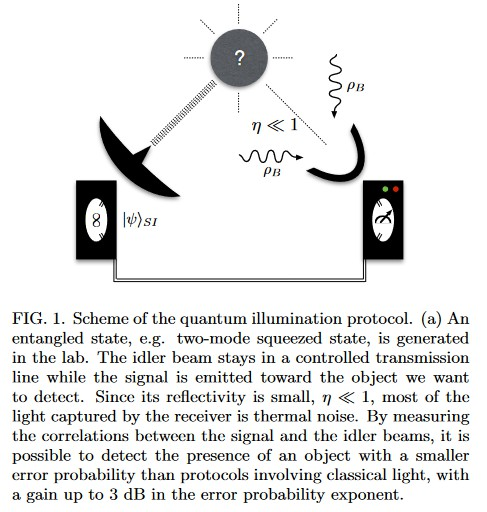
\includegraphics[scale=0.8]{chapters/quantum_information_research/quantum illumination.png}

Let us consider a general bipartite pure state representation of signal-ideler system written in the Schmidt decomposition form
\begin{align}
    \vert \psi \rangle_{SI}
    &= \sum_{\alpha} \sqrt{p_{\alpha}} \vert w_{\alpha} \rangle_S \vert v_{\alpha} \rangle_I.
\end{align}

In the Quantum Illumimation (QI) protocol, the signal modes of $M$ copies of $\vert \psi \rangle_{SI}$ are sent to the target region embedded in a bright thermal noise, in which there could possibly be an object. We receive $M$ copies of the state
\begin{align}
    \rho_{\eta}
    &= \tr_S\left[U_{\eta} \psi \bigotimes \rho_B U_{\eta}^{\dagger}\right],
\end{align}
where 
\begin{align}
    U_{\eta}
    &:= \exp[\sin^{-1}(\eta)(s^\dagger b - s b^\dagger)] \simeq \exp[\eta(s^\dagger b - s b^\dagger)]
    \label{def:U_eta}
\end{align}
is the signal-object interaction, modeled as a beamsplitter with amplitude reflectivity $\eta << 1$, and 
\begin{align}
\label{def: rho_B}
    \rho_B
    &:= \sum_n \frac{N_B^n}{(1+N_B)^{1+n}} \vert n \rangle \langle n \vert
\end{align} 
is the thermal state with mean photon number $N_B$.

In this framework, at the receiver side, $\eta=0$ corresponds to the absence of the object in the target region. We note $\eta$ is unknown parameter. So we measurement $\rho_{\eta}$ many times and get the estimation $\tilde{\eta}$. We then use $\hat{\eta}$ to determine whether is target is absent or present. This lie in the Estimation problem and state discrimination problem!


\subsection{Protocol}
The quantum illumination protocl has beed presented the last subsection. Here, we focus on the estimation protocol.

The main idea of the estimation protocol is to use QFI (\ref{def: qfi}) and CROB (\ref{def:crob}) for estimating $\eta$.

\begin{lemma}
    If a mode $s$ sent into a beamsplitter that has a thermal state input $b$ in the other port, then $U_{\eta} = \exp[\eta(s^\dagger b - s b^\dagger)]$ is indeed the unitary transformation.
    \label{lemma: unitary transformation}
\end{lemma}
\begin{proof}
    By the properties of matrix exponential \ref{def: matrix exponential}, we have
    \begin{align}
        U_{\eta}^{\dagger}
        &= \exp[\eta(s^\dagger b - s b^\dagger)]^\dagger \\
        &= \exp[\eta(b^\dagger s - b s^\dagger)].
    \end{align}
    Then we have
    \begin{align}
        U_{\eta} U_{\eta}^\dagger
        &= \exp\left[\eta(s^\dagger b - s b^\dagger + b^\dagger s - b s^\dagger)\right] \\
        &= \exp[\eta([s^\dagger, b] + [b^\dagger, s])] \\
        &\qquad\eqnote{By lemma \ref{lemma: communtation relations}} \nonumber \\
        &= \exp[\eta 0] \\
        &= \id.
    \end{align}
\end{proof}

\begin{lemma}
    The state $\rho_{\eta} = \tr_S \left[U_{\eta} \vert \psi\rangle \langle \psi \vert \otimes \rho_B U_{\eta}^{\dagger}\right]$, where $U_{\eta} \simeq \exp[\eta(s^\dagger b - s b^\dagger)]$. We have that the derivative computed at $\eta = 0$ is:
    \begin{align}
        \partial_{\eta} \rho_{\eta} = \tr_S[s^\dagger b - s b^\dagger, \vert \psi \rangle \langle \psi \vert \otimes \rho_B] = \sum_{\alpha \alpha^\prime} \sqrt{p_{\alpha} p_{\alpha'}} \vert v_{\alpha} \rangle \langle v_{\alpha} \vert \otimes \left[\langle w_{\alpha'} \vert s^\dagger \vert w_{\alpha} \rangle b - \langle w_{\alpha'} \vert s \vert w_{\alpha} \rangle b^\dagger, \rho_B \right].
    \end{align}
\end{lemma}
\begin{proof}
    \begin{align}
        \partial_{\eta} \rho_{\eta} \vert_{\eta=0}
        &= \tr_S\left[\partial_{\eta} U_{\eta} \vert \psi\rangle \langle \psi \vert \otimes \rho_B U_{\eta}^{\dagger}\right] \vert_{\eta=0} \\
        &= \tr_S\left[\partial_{\eta} \exp[\eta(s^\dagger b - s b^\dagger)] \vert \psi\rangle \langle \psi \vert \otimes \rho_B \exp[\eta(b^\dagger s - b s^\dagger)] \right] \vert_{\eta=0} \\
        &= \tr_S[ (s^\dagger b - s b^\dagger)\exp[\eta(s^\dagger b - s b^\dagger)] \vert \psi\rangle \langle \psi \vert \otimes \rho_B \exp[\eta(b^\dagger s - b s^\dagger)] +  \\
        &\exp[\eta(s^\dagger b - s b^\dagger)] \vert \psi\rangle \langle \psi \vert \otimes \rho_B \exp[\eta(b^\dagger s - b s^\dagger)](b^\dagger s - b s^\dagger) ]  \vert_{\eta=0}\\
        &= \tr_S[ (s^\dagger b - s b^\dagger) \vert \psi\rangle \langle \psi \vert \otimes \rho_B + \vert \psi\rangle \langle \psi \vert \otimes \rho_B (b^\dagger s - b s^\dagger) ]\\ 
        &= \tr_S[ (s^\dagger b - s b^\dagger) \vert \psi\rangle \langle \psi \vert \otimes \rho_B - \vert \psi\rangle \langle \psi \vert \otimes \rho_B (b s^\dagger - b^\dagger s) ]\\
        &\qquad\eqnote{By lemma \ref{lemma: communtation relations}} \nonumber \\
        &= \tr_S[ (s^\dagger b - s b^\dagger) \vert \psi\rangle \langle \psi \vert \otimes \rho_B - \vert \psi\rangle \langle \psi \vert \otimes \rho_B (s^\dagger b - s b^\dagger) ]\\
        &= \tr_S[s^\dagger b -s b^\dagger, \vert \psi \rangle \langle \psi \vert \otimes \rho_B].
    \end{align}
    Then we continue the derivation as
    \begin{align}
        &\tr_S\left[\vert \psi \rangle \langle \psi \vert \otimes \rho_B (s^\dagger b - s b^\dagger)\right]\\
        &= \tr\left[\vert \psi \rangle \langle \psi \rangle s^\dagger \otimes \rho_B b - \vert \psi \rangle \langle \psi \vert s \otimes \rho_B b^\dagger \right] \\
        &= \sum_k \langle w_k \vert \psi \rangle \langle \psi \vert s^\dagger \otimes \rho_B b \vert w_k \rangle - \sum_k \langle w_k \vert \psi \rangle \langle \psi \vert s \otimes \rho_B b \vert w_k \rangle \\
        &= \sum_{kij} \sqrt{p_i p_j} \langle w_k \vert \otimes I \vert w_i \rangle \langle w_j \vert \otimes \vert v_i \rangle \langle v_j \vert s^\dagger \otimes \id \vert w_k \rangle \otimes \id \otimes \rho_B b - \\
        &\sum_{kij} \sqrt{p_i p_j} \langle w_k \vert \otimes \id \vert w_i \rangle \langle w_j \vert \otimes \vert v_i \rangle \langle v_j \vert s \otimes \id \vert w_k \rangle \otimes \id \otimes \rho_B b^\dagger \\
        &= \sum_{kij} \sqrt{p_i p_j} \langle w_k \vert w_i \rangle \langle w_j \vert s^\dagger \vert w_k \rangle \otimes \vert v_i \rangle \langle v_j \vert \otimes \rho_B b - \\
        &\sum_{kij} \sqrt{p_i p_j} \langle w_k \vert w_i \rangle \langle w_j \vert s \vert w_k \rangle \otimes \vert v_i \rangle \langle v_j \vert \otimes  \rho_B b^\dagger \\
        &= \sum_{ij} \sqrt{p_i p_j} \langle w_j \vert s^\dagger \vert w_i \rangle \vert v_i \rangle \langle v_j \vert \otimes \rho_B b -
        \sum_{ij} \sqrt{p_i p_j} \langle w_j \vert s \vert w_i \rangle \vert v_i \rangle \langle v_j \vert \otimes  \rho_B b^\dagger \\
        &= \sum_{ij} \sqrt{p_i p_j} \vert v_i \rangle \langle v_j \vert \otimes \rho_B \langle w_j \vert s^\dagger \vert w_i \rangle b -
        \sum_{ij} \sqrt{p_i p_j}  \vert v_i \rangle \langle v_j \vert \otimes  \rho_B \langle w_j \vert s \vert w_i \rangle b^\dagger \\
        &= \sum_{ij} \sqrt{p_i p_j} \vert v_i \rangle \langle v_j \vert \otimes \rho_B \left[\langle w_j \vert s \vert w_i \rangle b^\dagger - \langle w_j \vert s^\dagger \vert w_i \rangle b \right].
    \end{align}
    Similarly, we can find that 
    \begin{align}
        &\tr_S\left[(s^\dagger b - s b^\dagger)\vert \psi \rangle \langle \psi \vert \otimes \rho_B\right]\\ 
        &= \sum_{ij} \left[\langle w_j \vert s^\dagger \vert w_i \rangle b - \langle w_j \vert s \vert w_i \rangle b^\dagger \right] \sqrt{p_i p_j} \vert v_i \rangle \langle v_j \vert \otimes \rho_B \\
        &= \sum_{ij} \sqrt{p_i p_j} \vert v_i \rangle \langle v_j \vert \otimes \left[\langle w_j \vert s^\dagger \vert w_i \rangle b - \langle w_j \vert s \vert w_i \rangle b^\dagger\right]\rho_B.
    \end{align}
    In summary, we have
    \begin{align}
        &\sum_{ij} \sqrt{p_i p_j} \vert v_i \rangle \langle v_j \vert \otimes \left[\left(\langle w_j \vert s^\dagger \vert w_i \rangle b - \langle w_j \vert s \vert w_i \rangle b^\dagger\right) \rho_B -  \left(\langle w_j \vert s \vert w_i \rangle b^\dagger - \langle w_j \vert s^\dagger \vert w_i \rangle b \right) \rho_B \right] \\
        &= \sum_{ij} \sqrt{p_i p_j} \vert v_i \rangle \langle v_j \vert \otimes \left[\left(\langle w_j \vert s^\dagger \vert w_i \rangle b - \langle w_j \vert s \vert w_i \rangle b^\dagger\right), \rho_B \right].
    \end{align}
\end{proof}

\begin{lemma}[$\rho_{\eta = 0}$]
    The states $\rho_{\eta=0}$ is derived as
    \begin{align}
        \rho_{\eta = 0}
        &= \sum_{\alpha} p_{\alpha} \vert v_{\alpha} \rangle \langle v_{\alpha} \vert \otimes \sum_n \frac{N_B^n}{(1 + N_B)^{1 + n}} \vert n \rangle \langle n \vert = \sum_{\alpha n} p_{\alpha} \frac{N_B^n}{(1+N_B)^{1+n}} \vert v_{\alpha} n \rangle \langle v_{\alpha } n \vert.
    \end{align}
\end{lemma}
\begin{proof}
    Recall the definition of $\rho_B$ in \ref{def: rho_B}, and that 
    \begin{align}
        \rho_{\eta}
        &= \tr_S\left[U_{\eta} \psi \otimes \rho_B U_{\eta}^\dagger \right] \\
        &\qquad\eqnote{Use lemma \ref{lemma: unitary transformation}} \nonumber \\
        &= \tr_S\left[\exp[\eta (s^\dagger b -s b^{\dagger}) \psi \otimes \rho_B \exp[\eta(b^\dagger s - b s^\dagger)]] \right].
    \end{align}
    Then we have
    \begin{align}
        \rho_{\eta = 0}
        &= \tr_S\left[\psi \otimes \rho_B \right]  \\
        &= \tr_S\left[\psi_{SI} \rangle \langle \psi_{SI} \vert \otimes \rho_B \right] \\
        &= \tr_S\left[\sum_{\alpha \beta} \sqrt{p_{\alpha} p_{\beta}} \vert w_{\alpha} \rangle \langle w_{\beta} \vert \otimes \vert v_{\alpha} \rangle \langle v_{\beta} \vert \otimes \rho_B \right] \\
        &= \sum_{\alpha \beta} \sqrt{p_{\alpha} p_{\beta}} \langle w_{\beta} \vert w_{\alpha} \rangle \vert v_{\alpha}\rangle \langle v_{\beta} \vert \otimes \rho_B \\
        &= \sum_{\alpha} p_{\alpha} \vert v_{\alpha} \rangle \langle v_{\alpha} \vert \otimes \rho_B.
    \end{align}
    Substitute $\rho_B$ into $\rho_{\eta=0}$, we arrive at the final result.
\end{proof}

\begin{definition}
    The quantum fisher information for the family of states $\rho_{\eta}$ is defined as
    \begin{align}
        H
        &= 2 \sum_{mn} \frac{\vert \langle \phi_m \vert (\partial \rho_{\eta})\vert_{\eta = 0} \vert \phi_n \rangle \vert^2}{\lambda_m \lambda_n},
    \end{align}
    where $\lambda_n$ is the eigenvalue of $\rho_{\eta = 0}$ corresponding to the eigenstate $\vert \phi_n \rangle$, and the derivativeis evaluated at $\eta = 0$.
\end{definition}

\begin{lemma}
\label{lemma: four results}
    Given the definition of $\rho_B$ \ref{def: rho_B}, we can compute the following four results:
    \begin{align}
        \langle n \vert b \rho_B \vert n^\prime \rangle 
        &= \rho_{n+1} \sqrt{n+1} \delta_{n+1, n^\prime} \\
        \langle n \vert b^\dagger \rho_B \vert n^\prime \rangle 
        &= \rho_{n^\prime} \sqrt{n^\prime + 1} \delta_{n, n^\prime + 1} \\
        \langle n \vert \rho_B b \vert n^\prime \rangle 
        &= \rho_n \sqrt{n+1} \delta_{n+1, n^\prime} \\
        \langle n \vert \rho_B b^\dagger \vert n \rangle 
        &= \rho_{n^\prime + 1} \sqrt{n^\prime + 1} \delta_{n, n^\prime + 1},
    \end{align}
    where $\rho_n = \frac{N_B^n}{(1 + N_B)^{1+n}}$.
\end{lemma}
\begin{proof}
    The first one:
    \begin{align}
        \langle n \vert b \rho_B \vert n^\prime \rangle 
        &= \langle n \vert b \sum_i \frac{N_B^i}{(1 + N_B)^{1+i}} \vert i \rangle \langle i \vert n^\prime \rangle \\
        &= \langle n \vert \sum_i \frac{N_B^i}{(1+N_B)^{1+i}} \sqrt{i} \vert i-1 \rangle \langle i \vert n^\prime \rangle \\
        &= \sum_i \frac{N_B^i}{(1 + N_B)^{1+i}} \sqrt{i} \langle n \vert i-1 \rangle \langle i \vert n^\prime \rangle \\
        &= \sum_i \frac{N_B^i}{(1 + N_B)^{1+i}} \sqrt{i} \delta_{n, i-1} \delta_{i, n^\prime} \\
        &= \frac{N_B^{n+1}}{(1 + N_B)^{1 + n+1}} \sqrt{n+1} \delta_{n+1, n^\prime} \\
        &= \rho_{n+1} \sqrt{n+1} \delta_{n+1, n^\prime}.
    \end{align}
    The second one:
    \begin{align}
        \langle n \vert b^\dagger \rho_B \vert n^\prime \rangle 
        &= \langle n \vert b^\dagger \sum_i \frac{N_B^i}{(1 + N_B)^{1+i}} \vert i \rangle \langle i \vert n^\prime \rangle \\
        &= \langle n \vert \sum_i \frac{N_B^i}{(1+N_B)^{1+i}} \sqrt{i+1} \vert i+1 \rangle \langle i \vert n^\prime \rangle \\
        &= \sum_i \frac{N_B^i}{(1 + N_B)^{1+i}} \sqrt{i+1} \langle n \vert i+1 \rangle \langle i \vert n^\prime \rangle \\
        &= \sum_i \frac{N_B^i}{(1 + N_B)^{1+i}} \sqrt{i+1} \delta_{n, i+1} \delta_{i, n^\prime} \\
        &= \sum_i \rho_i \sqrt{i+1} \delta_{n, i+1} \delta_{i, n^\prime} \\
        &= \rho_{n^\prime} \sqrt{n^\prime + 1} \delta_{n, n^\prime + 1}
    \end{align}
    The third one:
    \begin{align}
        \langle n \vert \rho_B b \vert n^\prime \rangle 
        &= \langle n \vert \sum_i \rho_i \vert i \rangle \langle i \vert b \vert n^\prime \rangle \\
        &= \langle n \vert \sum_i \rho_i \vert i \rangle (b^\dagger \vert i \rangle)^\dagger \vert n^\prime \rangle \\
        &= \langle n \vert \sum_i \rho_i \vert i \rangle (\sqrt{i+1} \vert i + 1\rangle)^\dagger \vert n^\prime \rangle \\
        &= \langle n \vert \sum_i \rho_i \vert i \rangle \langle i+1 \vert n^\prime \rangle \sqrt{i+1} \\
        &= \sum_i \rho_i \sqrt{i+1} \langle n \vert i \rangle \langle i+1 \vert n^\prime \rangle \\
        &= \sum_i \rho_i \sqrt{i+1} \delta_{n, i} \delta_{i+1, n^\prime}\\ 
        &= \rho_n \sqrt{n+1} \delta_{n+1, n^\prime}.
    \end{align}
    The fourth one:
    \begin{align}
        \langle n \vert \rho_B b^\dagger \vert n^\prime \rangle 
        &= \langle n \vert \sum_i \rho_i \vert i \rangle \langle i \vert b^\dagger \vert n^\prime \rangle \\
        &= \sum_i \rho_i \langle n \vert i \rangle \langle i \vert \sqrt{n^\prime + 1} \vert n^\prime + 1 \rangle \\
        &= \sum_i \rho_i \sqrt{n^\prime+1} \delta_{n, i} \delta_{i, n^\prime + 1} \\
        &= \rho_{n^\prime + 1} \sqrt{n^\prime + 1}\delta_{n, n^\prime + 1}.
    \end{align}
\end{proof}
\SZQ{Note that the resulting form can be different by apply $b$ or $b^\dagger$ in different direction.}

\begin{lemma}[Eq. (9) to Eq. (10)]
\label{lemma: 9 -> 10}
    We derive Eq. (10) from Eq. (9).
\end{lemma}
\begin{proof}
    We only need to focus on the numerator of the fraction 
    \begin{align}
        &\langle v_{\alpha}, n \vert \sum_{i j} \sqrt{p_i p_j} \vert v_i \rangle \langle v_j \vert \otimes \left[\langle w_j \vert s^\dagger \vert w_i \rangle b - \langle w_j \vert s \vert w_i \rangle  b^\dagger, \rho_B \right] \vert v_{\alpha^\prime}, n^\prime \rangle \\
        &= \sum_{ij} \sqrt{p_i p_j} \langle v_{\alpha}, n \vert v_i \rangle \langle v_j \vert \otimes \left[\langle w_j \vert s^\dagger \vert w_i \rangle b - \langle w_j \vert s \vert w_i \rangle b^\dagger, \rho_B \right] \vert v_{\alpha^\prime},n^\prime \rangle \\
        &= \sum_{ij} \sqrt{p_i p_j} \langle v_{\alpha} \vert v_i \rangle \langle v_j \vert v_{\alpha^\prime} \rangle \otimes \langle n \vert \left[\langle w_j \vert s^\dagger \vert w_i \rangle b - \langle w_j \vert s \vert w_i \rangle b^\dagger, \rho_B \right] \vert n^\prime \rangle \\
        &= \sqrt{p_{\alpha} p_{\alpha^{\prime}}} \langle n \vert \left[\langle w_j \vert s^\dagger \vert w_i \rangle b - \langle w_j \vert s \vert w_i \rangle b^\dagger, \rho_B \right] \vert n^\prime \rangle \\
        &=  \sqrt{p_{\alpha} p_{\alpha^{\prime}}} \langle n \vert \left[\langle w_j \vert s^\dagger \vert w_i \rangle b - \langle w_j \vert s \vert w_i \rangle b^\dagger, \rho_B \right] \vert n^\prime \rangle \\
        &= \sqrt{p_{\alpha} p_{\alpha^\prime}} \langle n \vert \left[ \langle w_j \vert s^\dagger \vert w_i \rangle b \rho_B - \langle w_j \vert s\vert w_i \rangle b^\dagger \rho_B - \langle w_j \vert s^\dagger \vert w_i \rangle \rho_B b + \langle w_j \vert s\vert w_i \rangle \rho_B b^\dagger  \right] \vert n^\prime \rangle \\
        &= \sqrt{p_{\alpha} p_{\alpha^\prime}} [\langle w_j \vert s^\dagger \vert w_i \rangle \langle n \vert b \rho_B \vert n^\prime \rangle - \langle w_j \vert s\vert w_i \rangle \langle n \vert b^\dagger \rho_B \vert n^\prime \rangle - \langle w_j \vert s^\dagger \vert w_i \rangle \langle n \vert \rho_B b \vert n^\prime \rangle \nonumber \\
        &+ \langle w_j \vert s\vert w_i \rangle \langle n \vert \rho_B b^\dagger \vert n^\prime \rangle ] \\
        &\qquad\eqnote{Use lemma } \nonumber \\
        &= \sqrt{p_{\alpha} p_{\alpha^\prime}} [\langle w_j \vert s^\dagger \vert w_i \rangle \rho_{n+1} \sqrt{n+1} \delta_{n+1, n^\prime} - \langle w_j \vert s \vert w_i \rangle \rho_{n^\prime} \sqrt{n^\prime + 1} \delta_{n, n^\prime + 1} \nonumber \\
        &- \langle w_j \vert s^\dagger \vert w_i \rangle \rho_n \sqrt{n+1}\delta_{n+1, n^\prime} + \langle w_j \vert s \vert w_i \rangle \rho_{n^\prime + 1} \sqrt{n^\prime + 1} \delta_{n, n^\prime + 1}] \\
        &= \sqrt{p_{\alpha} p_{\alpha^\prime}}[\langle w_j \vert s^\dagger \vert w_i \rangle (\rho_{n+1} - \rho_n)\sqrt{n+1}\delta_{n+1, n^\prime} \nonumber \\
        &- \langle w_j \vert s \vert w_i \rangle (\rho_{n^\prime} - \rho_{n^\prime + 1})\sqrt{n^\prime + 1}\delta_{n, n^\prime + 1}] \\
        &= \sqrt{p_{\alpha} p_{\alpha^\prime}}[\langle w_j \vert s^\dagger \vert w_i \rangle (\rho_{n^\prime} - \rho_n)\sqrt{n+1}\delta_{n+1, n^\prime}
        - \langle w_j \vert s \vert w_i \rangle (\rho_{n^\prime} - \rho_{n})\sqrt{n^\prime + 1}\delta_{n, n^\prime + 1}].
    \end{align}
\end{proof}


\begin{lemma}[Eq. (10) to Eq. (11)]
\label{lemma: 10 -> 11}
    We derive Eq. (11) from Eq. (10).
\end{lemma}
\begin{proof}
    \begin{align}
        &\vert \langle w_j \vert s^\dagger \vert w_i \rangle (\rho_{n^\prime} - \rho_n)\sqrt{n+1}\delta_{n+1, n^\prime}
        - \langle w_j \vert s \vert w_i \rangle (\rho_{n^\prime} - \rho_{n})\sqrt{n^\prime + 1}\delta_{n, n^\prime + 1} \vert^2 \\
        &= (\langle w_j \vert s^\dagger \vert w_i \rangle (\rho_{n^\prime} - \rho_n)\sqrt{n+1}\delta_{n+1, n^\prime}
        - \langle w_j \vert s \vert w_i \rangle (\rho_{n^\prime} - \rho_{n})\sqrt{n^\prime + 1}\delta_{n, n^\prime + 1}) \nonumber \\
        &(\langle w_j \vert s^\dagger \vert w_i \rangle (\rho_{n^\prime} - \rho_n)\sqrt{n+1}\delta_{n+1, n^\prime}
        - \langle w_j \vert s \vert w_i \rangle (\rho_{n^\prime} - \rho_{n})\sqrt{n^\prime + 1}\delta_{n, n^\prime + 1})^\dagger \\
        &= (\langle w_j \vert s^\dagger \vert w_i \rangle (\rho_{n^\prime} - \rho_n)\sqrt{n+1}\delta_{n+1, n^\prime}
        - \langle w_j \vert s \vert w_i \rangle (\rho_{n^\prime} - \rho_{n})\sqrt{n^\prime + 1}\delta_{n, n^\prime + 1}) \nonumber \\
        &(\langle w_j \vert s^\dagger \vert w_i \rangle^\dagger (\rho_{n^\prime} - \rho_n)\sqrt{n+1}\delta_{n+1, n^\prime}
        - \langle w_j \vert s \vert w_i \rangle^\dagger (\rho_{n^\prime} - \rho_{n})\sqrt{n^\prime + 1}\delta_{n, n^\prime + 1}) \\
        &= \vert \langle w_j \vert s^\dagger \vert w_i \rangle \vert^2(\rho_{n^\prime} - \rho_n)^2 (n+1) \delta_{n+1, n^\prime} + \vert \langle w_j \vert s \vert w_i \rangle \vert^2 (\rho_{n^\prime} - \rho_n)^2 (n^\prime + 1) \delta_{n, n^\prime + 1} \nonumber \\
        &- \langle w_j \vert s^\dagger \vert w_i \rangle (\rho_{n^\prime} - \rho_n)\sqrt{n+1}\delta_{n+1, n^\prime} \langle w_j \vert s \vert w_i \rangle^\dagger (\rho_{n^\prime} - \rho_{n})\sqrt{n^\prime + 1}\delta_{n, n^\prime + 1} \nonumber \\
        &- \langle w_j \vert s \vert w_i \rangle^\dagger (\rho_{n^\prime} - \rho_{n})\sqrt{n^\prime + 1}\delta_{n, n^\prime + 1} \langle w_j \vert s^\dagger \vert w_i \rangle^\dagger (\rho_{n^\prime} - \rho_n)\sqrt{n+1}\delta_{n+1, n^\prime} \\
        &= \vert \langle w_j \vert s^\dagger \vert w_i \rangle \vert^2(\rho_{n^\prime} - \rho_n)^2 (n+1) \delta_{n+1, n^\prime} + \vert \langle w_j \vert s \vert w_i \rangle \vert^2 (\rho_{n^\prime} - \rho_n)^2 (n^\prime + 1) \delta_{n, n^\prime + 1}.
    \end{align}
\end{proof}

\begin{lemma}
    We have $\vert \langle w_{\alpha^\prime} \vert s^\dagger \vert w_{\alpha} \rangle \vert^2 = \vert \langle w_{\alpha} \vert s \vert w_{\alpha^\prime} \rangle \vert^2$.
\end{lemma}

\begin{lemma}
    We have $\sum_{n} \frac{N_B^n}{(1 + N_B)^{1+n}} = 1$.
\end{lemma}
\begin{proof}
    \begin{align}
        \sum_{n=0}^{\infty} \frac{N_B^n}{(1 + N_B)^{1+n}}
        &= \frac{1}{1+N_B} \sum_{n} \frac{N_B^n}{(1+N_B)^n} \\
        &= \frac{1}{1+N_B} \sum_n \left(\frac{N_B}{1+N_B}\right)^n \\
        &= \frac{1}{1+N_B} \cdot \frac{1}{1 - \frac{N_B}{1+N_B}} \\
        &= \frac{1}{1+N_B} \cdot (1 + N_B) \\
        &= 1.
    \end{align}
\end{proof}

\begin{lemma}[Eq. (11) to Eq. (12)]
\label{lemma: 11 -> 12}
    We derive Eq. (12) from Eq. (11).
\end{lemma}
\begin{proof}
    \begin{align}
        \cdots
        &= 2 \sum_{\alpha \alpha^\prime n n^\prime} \frac{p_{\alpha} p_{\alpha^\prime} (\rho_{n^\prime} - \rho_n)^2}{p_{\alpha} \rho_{n} + p_{\alpha^\prime} \rho_{n^\prime}} \vert \langle w_{\alpha^\prime} \vert s^\dagger \vert w_{\alpha} \rangle \vert^2 (n+1) \delta_{n^\prime, n+1} \nonumber \\
        &+ 2 \sum_{\alpha \alpha^\prime n n^\prime} \frac{p_{\alpha} p_{\alpha^\prime} (\rho_{n^\prime} - \rho_n)^2}{p_{\alpha} \rho_{n} + p_{\alpha^\prime} \rho_{n^\prime}} \vert \langle w_{\alpha^\prime} \vert s \vert w_{\alpha} \rangle \vert^2 (n^\prime + 1) \delta_{n, n^\prime+1} \\
        &= 2 \sum_{\alpha \alpha^\prime n} \frac{p_{\alpha} p_{\alpha^\prime} (\rho_{n+1} - \rho_n)^2}{p_{\alpha} \rho_{n} + p_{\alpha^\prime} \rho_{n+1}} \vert \langle w_{\alpha^\prime} \vert s^\dagger \vert w_{\alpha} \rangle \vert^2 (n+1) \nonumber \\
        &+ 2 \sum_{\alpha \alpha^\prime n^\prime} \frac{p_{\alpha} p_{\alpha^\prime} (\rho_{n^\prime} - \rho_{n^\prime + 1})^2}{p_{\alpha} \rho_{n^\prime + 1} + p_{\alpha^\prime} \rho_{n^\prime}} \vert \langle w_{\alpha^\prime} \vert s \vert w_{\alpha} \rangle \vert^2 (n^\prime + 1) \\
        &= 2 \sum_{\alpha \alpha^\prime n} \frac{p_{\alpha} p_{\alpha^\prime} (\rho_{n+1} - \rho_n)^2}{p_{\alpha} \rho_{n} + p_{\alpha^\prime} \rho_{n+1}} \vert \langle w_{\alpha^\prime} \vert s^\dagger \vert w_{\alpha} \rangle \vert^2 (n+1) \nonumber \\
        &+ 2 \sum_{\alpha \alpha^\prime n} \frac{p_{\alpha} p_{\alpha^\prime} (\rho_{n} - \rho_{n + 1})^2}{p_{\alpha} \rho_{n + 1} + p_{\alpha^\prime} \rho_{n}} \vert \langle w_{\alpha^\prime} \vert s \vert w_{\alpha} \rangle \vert^2 (n + 1) \\
        &= 2 \sum_{\alpha \alpha^\prime n} (n+1) p_{\alpha} p_{\alpha^\prime} (\rho_{n+1} - \rho_n)^2 \left[\frac{\vert \langle w_{\alpha^\prime} \vert s^\dagger \vert w_{\alpha} \rangle \vert^2}{p_{\alpha} \rho_n + p_{\alpha^\prime} \rho_{n+1}} + \frac{\vert \langle w_{\alpha^\prime} \vert s \vert w_{\alpha} \rangle \vert^2}{p_{\alpha } \rho_{n+1} + p_{\alpha^\prime} \rho_n} \right]
    \end{align}
\end{proof}

\begin{lemma}
\label{lemma: power series}
    \begin{align}
        \sum_{n} (n+1) \frac{N_B^n}{(1+N_B)^{1+n}} = 1 + N_B.
    \end{align}
\end{lemma}
\begin{proof}
    We define
    \begin{align}
        f(x)
        &:= \sum_{n=0}^{\infty} N_B^n x^{n+1}.
    \end{align}
    We have
    \begin{align}
        f(x) = x \sum_n (N_B x)^n = \frac{x}{1 - N_B x},
    \end{align}
    and 
    \begin{align}
        f^{\prime}(x) = \frac{(1-N_B x) - x (-N_B)}{(1 - N_B x)^2} = \frac{1}{(1-N_B x)^2}
    \end{align}
    We also have
    \begin{align}
        f^\prime(x) = \sum_{n=0}^{\infty} N_B^n (n+1) x^{n}.
    \end{align}
    Then, 
    \begin{align}
        f^{\prime}\left(\frac{1}{1+N_B}\right)
        = \sum_{n} (n+1) \frac{N_B^n}{(1+N_B)^n} 
        &=  (1+N_B) \sum_{n} (n+1) \frac{N_B^n}{(1+N_B)^{1+n}} \\
        &= \frac{1}{(1 - N_B \frac{1}{1+N_B})^2} \\
        &= (1 + N_B)^2.
    \end{align}
    Thus, we have
    \begin{align}
        \sum_{n} (n+1) \frac{N_B^n}{(1+N_B)^{1+n}} = 1 + N_B.
    \end{align}
\end{proof}

\begin{lemma}[Eq. (12) to Eq. (14)]
\label{lemma: 12 -> 14}
    We derive Eq. (14) from Eq. (12).
\end{lemma}
\begin{proof}
\begin{align}
    &2 \sum_{\alpha \alpha^\prime n} \frac{p_{\alpha} p_{\alpha^\prime} (\rho_{n+1} - \rho_n)^2}{p_{\alpha} \rho_{n} + p_{\alpha^\prime} \rho_{n+1}} \vert \langle w_{\alpha^\prime} \vert s^\dagger \vert w_{\alpha} \rangle \vert^2 (n+1) \nonumber \\
    &+ 2 \sum_{\alpha \alpha^\prime n} \frac{p_{\alpha} p_{\alpha^\prime} (\rho_{n} - \rho_{n + 1})^2}{p_{\alpha} \rho_{n + 1} + p_{\alpha^\prime} \rho_{n}} \vert \langle w_{\alpha^\prime} \vert s \vert w_{\alpha} \rangle \vert^2 (n + 1) \\
    &= 2 \sum_{ \alpha^\prime \alpha n} \frac{ p_{\alpha^\prime} p_{\alpha} (\rho_{n+1} - \rho_n)^2}{p_{\alpha^\prime} \rho_{n} + p_{\alpha} \rho_{n+1}} \vert \langle w_{\alpha} \vert s^\dagger \vert w_{\alpha^\prime} \rangle \vert^2 (n+1) \nonumber \\
    &+ 2 \sum_{\alpha \alpha^\prime n} \frac{p_{\alpha} p_{\alpha^\prime} (\rho_{n} - \rho_{n + 1})^2}{p_{\alpha} \rho_{n + 1} + p_{\alpha^\prime} \rho_{n}} \vert \langle w_{\alpha^\prime} \vert s \vert w_{\alpha} \rangle \vert^2 (n + 1) \\
    &= 2 \sum_{ \alpha^\prime \alpha n} \frac{ p_{\alpha^\prime} p_{\alpha} (\rho_{n+1} - \rho_n)^2}{p_{\alpha^\prime} \rho_{n} + p_{\alpha} \rho_{n+1}} \vert \langle w_{\alpha^\prime} \vert s \vert w_{\alpha} \rangle \vert^2 (n+1) \nonumber \\
    &+ 2 \sum_{\alpha \alpha^\prime n} \frac{p_{\alpha} p_{\alpha^\prime} (\rho_{n} - \rho_{n + 1})^2}{p_{\alpha} \rho_{n + 1} + p_{\alpha^\prime} \rho_{n}} \vert \langle w_{\alpha^\prime} \vert s \vert w_{\alpha} \rangle \vert^2 (n + 1) \\
    &= 4 \sum_{\alpha \alpha^\prime n} (n+1) p_{\alpha} p_{\alpha^\prime} (\rho_{n+1} - \rho_n)^2 \frac{\vert \langle w_{\alpha^\prime} \vert s \vert w_{\alpha} \rangle \vert^2}{p_{\alpha} \rho_{n+1} + p_{\alpha^\prime} \rho_n} \\
    &= 4 \sum_{\alpha \alpha^\prime n} (n+1) p_{\alpha} p_{\alpha^\prime} \rho_n^2 (\frac{\rho_{n+1}}{\rho_n} - 1)^2 \frac{\vert \langle w_{\alpha^\prime} \vert s \vert w_{\alpha} \rangle \vert^2}{p_{\alpha} \rho_{n+1} + p_{\alpha^\prime} \rho_n} \\
    &= 4 \sum_{\alpha \alpha^\prime n} (n+1) p_{\alpha} p_{\alpha^\prime} \rho_n \left(\frac{\rho_{n+1}}{\rho_n} - 1\right)^2 \frac{\vert \langle w_{\alpha^\prime} \vert s \vert w_{\alpha} \rangle \vert^2}{p_{\alpha} \frac{\rho_{n+1}}{\rho_n} + p_{\alpha^\prime}} \\
    &\qquad\eqnote{By def.} \nonumber \\
    &= 4 \sum_{\alpha \alpha^\prime n} (n+1) p_{\alpha} p_{\alpha^\prime} \rho_n \left(\frac{N_B}{1+N_B} - 1\right)^2 \frac{\vert \langle w_{\alpha^\prime} \vert s \vert w_{\alpha} \rangle \vert^2}{p_{\alpha} \frac{N_B}{1+1N_B} + p_{\alpha^\prime}} \\
    &= 4 \sum_{n} (n+1) \frac{N_B^n}{(1+N_B)^{1+n}} \cdot \frac{1}{(1+N_B)^2} \sum_{\alpha \alpha^\prime} \frac{p_{\alpha} p_{\alpha^\prime}}{p_{\alpha} \frac{N_B}{1+N_B} + p_{\alpha^\prime}} \vert \langle w_{\alpha^\prime} \vert s\vert w_{\alpha} \rangle \vert^2 \\
    &= \frac{4}{(1+N_B)^2} \sum_{n} (n+1) \frac{N_B^n}{(1+N_B)^{1+n}} \sum_{\alpha \alpha^\prime} \frac{p_{\alpha} p_{\alpha^\prime}}{p_{\alpha} \frac{N_B}{1+N_B} + p_{\alpha^\prime}} \vert \langle w_{\alpha^\prime} \vert s\vert w_{\alpha} \rangle \vert^2 \\
    &\qquad\eqnote{Use lemma \ref{lemma: power series}} \nonumber \\
    &= \frac{4}{(1+N_B)^2} (1+N_B) \sum_{\alpha \alpha^\prime} \frac{p_{\alpha} p_{\alpha^\prime}}{p_{\alpha} \frac{N_B}{1+N_B} + p_{\alpha^\prime}} \vert \langle w_{\alpha^\prime} \vert s\vert w_{\alpha} \rangle \vert^2 \\
    &= \frac{4}{(1+N_B)} \sum_{\alpha \alpha^\prime} \frac{p_{\alpha} p_{\alpha^\prime}}{p_{\alpha} \frac{N_B}{1+N_B} + p_{\alpha^\prime}} \vert \langle w_{\alpha^\prime} \vert s\vert w_{\alpha} \rangle \vert^2.
\end{align}
\end{proof}

\begin{lemma}[The QFI for the returned state $\rho_{\eta}$ in Eq. (3) \cite{sanz2017quantum}]
    \label{lemma: qfi of returned state}
    The QFI for $\rho_{\eta}$ is
    \begin{align}
        H
        &:= \frac{4}{1+N_B} \sum_{\alpha \alpha^\prime} \frac{p_\alpha p_{\alpha^\prime}}{p_{\alpha^\prime} + p_{\alpha} \frac{N_B}{1+N_B}} \vert \langle w_{\alpha^\prime} \vert s \vert w_{\alpha} \rangle \vert^2.
    \end{align}
\end{lemma}
\begin{proof}
    \begin{align}
        H
        &= 2 \sum_{\alpha \alpha^\prime n n^\prime} \frac{\left\vert \langle v_{\alpha}, n \vert \sum_{i j} \sqrt{p_{i} P_{j}} \vert v_i \rangle \langle v_j \vert \otimes [\langle w_j \vert s^\dagger \vert w_i \rangle b - \langle w_j \vert s \vert w_i \rangle b^\dagger, \rho_{\rm th}] \vert v_{\alpha^\prime}, n^\prime \rangle \vert \right\vert^2}{p_{\alpha} \rho_n + p_{\alpha^\prime} \rho_{n^\prime}} \\
        &\qquad\eqnote{Use lemma \ref{lemma: 9 -> 10}} \nonumber \\
        &= 2 \sum_{\alpha \alpha^\prime n n^\prime} \frac{p_{\alpha} p_{\alpha^\prime}\vert \langle w_j \vert s^\dagger \vert w_i \rangle (\rho_{n^\prime} - \rho_n)\sqrt{n+1}\delta_{n+1, n^\prime}
        - \langle w_j \vert s \vert w_i \rangle (\rho_{n^\prime} - \rho_{n})\sqrt{n^\prime + 1}\delta_{n, n^\prime + 1}\vert^2}{p_{\alpha} \rho_n + p_{\alpha^\prime} \rho_{n^\prime}} \\
        &\qquad\eqnote{Use lemma \ref{lemma: 10 -> 11}} \nonumber \\
        &= 2 \sum_{\alpha \alpha^\prime n n^\prime} \frac{p_{\alpha} p_{\alpha^\prime} (\rho_{n^\prime} - \rho_n)^2}{p_{\alpha} \rho_n + p_{\alpha^\prime} \rho_{n^\prime}} \nonumber \\
        &\left(\vert \langle w_j \vert s^\dagger \vert w_i \rangle \vert^2(\rho_{n^\prime} - \rho_n)^2 (n+1) \delta_{n+1, n^\prime} + \vert \langle w_j \vert s \vert w_i \rangle \vert^2 (\rho_{n^\prime} - \rho_n)^2 (n^\prime + 1) \delta_{n, n^\prime + 1}\right) \\
        &\qquad\eqnote{Use lemma \ref{lemma: 11 -> 12}} \nonumber \\
        &= 2 \sum_{\alpha \alpha^\prime n} (n+1) p_{\alpha} p_{\alpha^\prime} (\rho_{n+1} - \rho_n)^2 \left[\frac{\vert \langle w_{\alpha^\prime} \vert s^\dagger \vert w_{\alpha} \rangle \vert^2}{p_{\alpha} \rho_n + p_{\alpha^\prime} \rho_{n+1}} + \frac{\vert \langle w_{\alpha^\prime} \vert s \vert w_{\alpha} \rangle \vert^2}{p_{\alpha } \rho_{n+1} + p_{\alpha^\prime} \rho_n} \right] \\
        &\qquad\eqnote{Use lemma \ref{lemma: 12 -> 14}} \nonumber \\
        &= \frac{4}{(1+N_B)} \sum_{\alpha \alpha^\prime} \frac{p_{\alpha} p_{\alpha^\prime}}{p_{\alpha} \frac{N_B}{1+N_B} + p_{\alpha^\prime}} \vert \langle w_{\alpha^\prime} \vert s\vert w_{\alpha} \rangle \vert^2.
    \end{align}
\end{proof}

\begin{definition}
    Define $N_S:= \sum_{\alpha} p_{\alpha} \langle w_{\alpha} \vert s^\dagger s \vert w_{\alpha} \rangle$.
\end{definition}

\begin{lemma}
    We have
    \begin{align}
        H \leq \frac{4 N_S}{1+N_B}.
    \end{align}
\end{lemma}
\begin{proof}
    \begin{align}
        H
        &\leq \frac{4}{1+N_B} \sum_{\alpha \alpha^\prime} p_{\alpha} \langle w_{\alpha} \vert s^\dagger \vert w_{\alpha^\prime} \rangle \langle w_{\alpha^\prime} \vert s \vert w_{\alpha} \rangle  \\
        &= \frac{4}{1+N_B} \sum_{\alpha} p_{\alpha} \langle w_{\alpha} s^\dagger s \vert w_{\alpha} \rangle \\
        &= \frac{4 N_S}{1+N_B}.
    \end{align}
\end{proof}

\begin{lemma}
    We have following inequality
    \begin{align}
        \frac{p_{\alpha^\prime} + p_{\alpha} \frac{N_B}{1+N_B}}{p_{\alpha} p_{\alpha^\prime}} 
        &\geq \frac{1}{\sqrt{\frac{1+N_B}{N_B}} \left(\frac{p_{\alpha} + p_{\alpha^\prime}}{4}\right)}
    \end{align}
\end{lemma}
\begin{proof}
\begin{align}
    \frac{p_{\alpha^\prime} + p_{\alpha} \frac{N_B}{1+N_B}}{p_{\alpha} p_{\alpha^\prime}} 
    &= \frac{1}{p_{\alpha}} + \frac{\frac{N_B}{1+N_B}}{p_{\alpha^\prime}}  \\
    &\geq 2 \sqrt{\frac{\frac{N_B}{1+N_B}}{p_{\alpha} p_{\alpha^\prime}}} \\
    &= 2 \sqrt{\frac{N_B}{1+N_B}} \sqrt{\frac{1}{p_{\alpha} p_{\alpha^\prime}}} \\
    &\geq 2 \sqrt{\frac{N_B}{1+N_B}} \frac{2}{p_{\alpha} + p_{\alpha^\prime}} \\
    &= \sqrt{\frac{N_B}{1+N_B}} \frac{4}{p_{\alpha} p_{\alpha^\prime}}.
\end{align}    
\end{proof}

\begin{lemma}
    We derive
    \begin{align}
        H 
        &\leq \frac{2N_S + 1}{N_B}.
    \end{align}
\end{lemma}
\begin{proof}
\begin{align}
    H 
    &= \frac{4}{1+N_B} \sum_{\alpha \alpha^\prime} \frac{p_{\alpha} p_{\alpha^\prime}}{p_{\alpha^\prime} + p_{\alpha} \frac{N_B}{1+N_B}} \vert \langle w_{\alpha^\prime} \vert s \vert w_{\alpha} \rangle \vert^2 \\
    &\leq \frac{4}{1+N_B} \sum_{\alpha \alpha^\prime} \sqrt{\frac{N_B+1}{N_B}}\frac{p_{\alpha} + p_{\alpha^\prime}}{4} \vert \langle w_{\alpha^\prime} \vert s \vert w_{\alpha} \rangle \vert^2 \\
    &\leq \frac{4}{1+N_B} \sum_{\alpha \alpha^\prime} \frac{N_B+1}{N_B} \frac{p_{\alpha} + p_{\alpha^\prime}}{4} \vert \langle w_{\alpha^\prime} \vert s \vert w_{\alpha} \rangle \vert^2 \\
    &= \frac{1}{N_B} \sum_{\alpha \alpha^\prime} (p_{\alpha} + p_{\alpha^\prime}) \vert \langle w_{\alpha^\prime} \vert s \vert w_{\alpha} \rangle \vert^2 \\
    &= \frac{1}{N_B} \left[ \sum_{\alpha \alpha^\prime} p_{\alpha} \vert \langle w_{\alpha^\prime} \vert s \vert w_{\alpha} \rangle \vert^2 + \sum_{\alpha \alpha^\prime} p_{\alpha^\prime} \vert \langle w_{\alpha^\prime} \vert s \vert w_{\alpha} \rangle \vert^2\right] \\
    &= \frac{1}{N_B} \left[ \sum_{\alpha \alpha^\prime} p_{\alpha} \langle w_{\alpha^\prime} \vert s \vert w_{\alpha} \rangle \langle w_{\alpha} \vert s^\dagger \vert w_{\alpha^\prime} \rangle  + \sum_{\alpha \alpha^\prime} p_{\alpha^\prime} \langle w_{\alpha^\prime} \vert s \vert w_{\alpha} \rangle \langle w_{\alpha} \vert s^\dagger \vert w_{\alpha^\prime} \rangle \right] \\
    &= \frac{1}{N_B}\left[\sum_{\alpha} p_{\alpha} \langle w_{\alpha} \vert s^\dagger s \vert w_{\alpha} \rangle + \sum_{\alpha^\prime} p_{\alpha^\prime} \langle w_{\alpha^\prime} \vert s s^\dagger \vert w_{\alpha^\prime} \rangle\right] \\
    &= \frac{1}{N_B}\left[\sum_{\alpha} p_{\alpha} \langle w_{\alpha} \vert s^\dagger s \vert w_{\alpha} \rangle + \sum_{\alpha^\prime} p_{\alpha^\prime} \langle w_{\alpha^\prime} \vert s^\dagger s +1 \vert w_{\alpha^\prime} \rangle\right] \\
    &= \frac{1}{N_B} \left[2 N_S + 1\right] \\
    &= \frac{2 N_S + 1}{N_B}.
\end{align}
\end{proof}

\begin{definition}
    The symmetric logarithmic derivative of $\rho_{\eta}$ computed as $\eta = 0$ is 
    \begin{align}
        \hat{L}
        &= 2 \sum_{m n} \frac{\langle \phi_{m} \vert (\partial_{\eta} \rho_{\eta})\vert_{\eta = 0}\vert \phi_n \rangle}{\lambda_m + \lambda_n} \vert \phi_m \rangle \langle \phi_n \vert.
    \end{align}
\end{definition}

\begin{lemma}[\cite{bennett1993teleporting}]
    A possible estimator saturating Eq. (2) is given by the mean of the $M$ single-copy measurement outcomes of the observable $\hat{O} = \frac{\hat{L}}{H}$. This estimator is optimal for evaluating the reflective parametric in the assumed neighborhood of zero.
\end{lemma}

\begin{lemma}
    The optimal observable is given by $\hat{O} = \frac{\hat{L}}{H}$. We thus have
    \begin{align}
        \hat{O}
        &= -\frac{2}{H(1+N_B)} \sum_{\alpha \alpha^\prime} \vert v_{\alpha} \rangle \langle v_{\alpha^\prime} \vert \otimes \left(c^\ast_{\alpha \alpha^\prime} b + c_{\alpha^\prime \alpha} b^\dagger \right),
    \end{align}
    where we have introduced the quantity 
    \begin{align}
        c_{\alpha \alpha^\prime} 
        &\equiv \frac{\sqrt{p_{\alpha} p_{\alpha^\prime}\langle w_{\alpha} \vert s \vert w_{\alpha^\prime} \rangle}}{p_{\alpha} + p_{\alpha^\prime} \frac{N_B}{1+N_B}}.
    \end{align}
\end{lemma}
\begin{proof}
    The proof is similar to the proof of $H$. Unlike previous derive, we merge all the proof into one this time.
    \begin{align}
        \tilde{L}
        &= 2 \sum_{\alpha \alpha^\prime n n^\prime} \langle v_{\alpha}, n \vert \sum_{\beta \beta^\prime} \sum_{\beta \beta^\prime} \sqrt{p_{\beta} p_{\beta^\prime}} \vert v_{\beta} \rangle \langle v_{\beta^\prime} \otimes [\langle w_{\beta^\prime} \vert s^\dagger \vert w_{\beta} \rangle b - \langle w_{\beta^\prime} \vert s \vert w_{\beta} \rangle b^\dagger, \rho_B] \vert v_{\alpha^\prime}, n^\prime \rangle \nonumber \\
        &\vert v_{\alpha}, n \rangle \langle v_{\alpha^\prime}, n^\prime \vert \\
        &= 2 \sum_{\alpha \alpha^\prime n n^\prime \beta \beta^\prime} \sqrt{p_{\beta} p_{\beta^\prime}} \langle v_{\alpha} \vert v_{\beta} \rangle \langle v_{\beta^\prime} \vert v_{\alpha^\prime} \rangle \otimes \langle n \vert [\langle w_{\beta^\prime} \vert s^\dagger \vert w_{\beta} \rangle b - \langle w_{\beta^\prime} \vert s \vert w_{\beta} \rangle b^\dagger, \rho_B] \vert n^\prime \nonumber \\
        &\vert v_{\alpha}, n \rangle \langle v_{\alpha^\prime}, n^\prime \vert \\
        &= 2 \sum_{\alpha \alpha^\prime n n^\prime} \sqrt{p_{\alpha} p_{\alpha^\prime}} \langle n \vert [\langle w_{\beta^\prime} \vert s^\dagger \vert w_{\beta} \rangle b - \langle w_{\beta^\prime} \vert s \vert w_{\beta} \rangle b^\dagger, \rho_B] \vert n^\prime \rangle \cdots \\
        &= 2 \sum_{\alpha \alpha^\prime n n^\prime} \sqrt{p_{\alpha} p_{\alpha^\prime}} [ (\langle w_{\alpha^\prime} \vert s^\dagger \vert w_{\alpha} \langle n \vert b \rho_B \vert n^\prime \rangle - \langle w_{\alpha^\prime} \vert s \vert w_{\alpha} \rangle \langle n \vert b^\dagger \rho_B \vert n^\prime \rangle) \nonumber \\
        &- (\langle w_{\alpha^\prime} \vert s^\dagger \vert w_{\alpha} \rangle \langle n \rho_B b \vert n^\prime \rangle - \langle w_{\alpha^\prime} \vert s \vert w_{\alpha} \rangle \langle n \rho_B b^\dagger \vert n^\prime \rangle) ] \\
        &= 2 \sum_{\alpha \alpha^\prime n n^\prime} \sqrt{p_{\alpha} p_{\alpha^\prime}} [\langle w_{\alpha^\prime} \vert s^\dagger \vert w_{\alpha} \rangle(\rho_{n+1} - \rho_n) \sqrt{n+1} \delta_{n+1, n^\prime} - \langle w_{\alpha^\prime} \vert s \vert w_{\alpha} \rangle \nonumber \\
        &(\rho_{n^\prime} - \rho_{n^\prime + 1}) \sqrt{n^\prime + 1}\delta_{n,n^\prime+1}] \cdots \\
        &= 2 \sum_{\alpha \alpha^\prime n n^\prime} \sqrt{p_{\alpha} p_{\alpha^\prime}} [\langle w_{\alpha^\prime} \vert s^\dagger \vert w_{\alpha} \rangle(\rho_{n^\prime} - \rho_n) \sqrt{n+1} \delta_{n+1, n^\prime} - \langle w_{\alpha^\prime} \vert s \vert w_{\alpha} \rangle \nonumber \\
        &(\rho_{n^\prime} - \rho_{n}) \sqrt{n^\prime + 1}\delta_{n,n^\prime+1}] \cdots \\
        &= 2 \sum_{\alpha \alpha^\prime n n^\prime} \sqrt{p_{\alpha} p_{\alpha^\prime}} (\rho_{n^\prime} - \rho_n) \left[\langle w_{\alpha^\prime} \vert s^\dagger \vert w_{\alpha} \rangle \sqrt{n+1} \delta_{n+1, n^\prime} - \langle w_{\alpha^\prime} \vert s \vert w_{\alpha} \rangle
        \sqrt{n^\prime + 1}\delta_{n,n^\prime+1}\right] \cdots \\
        &= 2 \sum_{\alpha \alpha^\prime n n^\prime} \sqrt{p_{\alpha} p_{\alpha^\prime}} (\rho_{n^\prime} - \rho_n) \langle w_{\alpha^\prime} \vert s^\dagger \vert w_{\alpha} \rangle \sqrt{n+1} \delta_{n+1, n^\prime} \cdots - \nonumber \\
        &2 \sum_{\alpha \alpha^\prime n n^\prime} \sqrt{p_{\alpha} p_{\alpha^\prime}} (\rho_{n^\prime} - \rho_n) \langle w_{\alpha^\prime} \vert s \vert w_{\alpha} \rangle \sqrt{n^\prime + 1} \delta_{n, n^\prime + 1} \cdots \\
        &= 2 \sum_{\alpha \alpha^\prime n} \sqrt{p_{\alpha} p_{\alpha^\prime}} (\rho_{n+1} - \rho_n) \langle w_{\alpha^\prime} \vert s^\dagger \vert w_{\alpha} \rangle \sqrt{n+1} \cdots - 2 \sum_{\alpha \alpha^\prime n^\prime} \sqrt{p_{\alpha} p_{\alpha^\prime}} (\rho_{n^\prime} - \rho_{n^\prime + 1}) \langle w_{\alpha^\prime} \vert s \vert w_{\alpha} \rangle \sqrt{n^\prime + 1} \\
        &= 2 \sum_{\alpha \alpha^\prime n} \sqrt{p_{\alpha} p_{\alpha^\prime}} (\rho_{n+1} - \rho_n) \langle w_{\alpha^\prime} \vert s^\dagger \vert w_{\alpha} \rangle \sqrt{n+1} \cdots - 2 \sum_{\alpha \alpha^\prime n} \sqrt{p_{\alpha} p_{\alpha^\prime}} (\rho_{n} - \rho_{n + 1}) \langle w_{\alpha^\prime} \vert s \vert w_{\alpha} \rangle \sqrt{n + 1} \\
        &= 2 \sum_{\alpha \alpha^\prime n} \sqrt{p_{\alpha} p_{\alpha^\prime}} (\rho_{n+1} - \rho_n) \left(\langle w_{\alpha^\prime} \vert s^\dagger \vert w_{\alpha} \rangle + \langle w_{\alpha^\prime} \vert s \vert w_{\alpha} \rangle \right) \sqrt{n+1} \\
        &= 2 \sum_{\alpha \alpha^\prime n} \sqrt{p_{\alpha} p_{\alpha^\prime}} \sqrt{n+1} (\rho_{n+1} - \rho_n) \langle w_{\alpha} \vert s \vert w_{\alpha^\prime} \rangle^\ast
        + 2 \sum_{\alpha \alpha^\prime n} \sqrt{p_{\alpha} p_{\alpha^\prime}} \sqrt{n+1} (\rho_{n+1} - \rho_n) \langle w_{\alpha} \vert s \vert w_{\alpha^\prime} \rangle.
    \end{align}
    Thus, we have
    \begin{align}
        L
        &= 2 \sum_{\alpha \alpha^\prime n} \sqrt{p_{\alpha} p_{\alpha^\prime}} \sqrt{n+1} (\rho_{n+1} - \rho_n) \frac{\langle w_{\alpha} \vert s \vert w_{\alpha^\prime} \rangle^\ast}{p_{\alpha} \rho_{n+1} + p_{\alpha^\prime} \rho_n}
        + 2 \sum_{\alpha \alpha^\prime n} \sqrt{p_{\alpha} p_{\alpha^\prime}} \sqrt{n+1} (\rho_{n+1} - \rho_n) \frac{\langle w_{\alpha} \vert s \vert w_{\alpha^\prime} \rangle}{p_{\alpha} \rho_{n+1} + p_{\alpha^\prime} \rho_n} \\
        &= 2 \sum_{\alpha \alpha^\prime n} \sqrt{p_{\alpha} p_{\alpha^\prime}} \sqrt{n+1} (1 - \frac{\rho_{n}}{\rho_{n+1}}) \frac{\langle w_{\alpha} \vert s \vert w_{\alpha^\prime} \rangle^\ast}{p_{\alpha} + p_{\alpha^\prime} \frac{\rho_n}{\rho_{n+1}}}
        + 2 \sum_{\alpha \alpha^\prime n} \sqrt{p_{\alpha} p_{\alpha^\prime}} \sqrt{n+1} (1 - \frac{\rho_{n}}{\rho_{n+1}}) \frac{\langle w_{\alpha} \vert s \vert w_{\alpha^\prime} \rangle}{p_{\alpha} + p_{\alpha^\prime} \frac{\rho_n}{\rho_{n+1}}} \\
        &= 2 \sum_{\alpha \alpha^\prime n} \sqrt{p_{\alpha} p_{\alpha^\prime}} \sqrt{n+1} (1 - \frac{N_B}{N_B+1}) \frac{\langle w_{\alpha} \vert s \vert w_{\alpha^\prime} \rangle^\ast}{p_{\alpha} + p_{\alpha^\prime} \frac{N_B}{N_B+1}}
        + 2 \sum_{\alpha \alpha^\prime n} \sqrt{p_{\alpha} p_{\alpha^\prime}} \sqrt{n+1} (1 - \frac{N_B}{N_B+1}) \frac{\langle w_{\alpha} \vert s \vert w_{\alpha^\prime} \rangle}{p_{\alpha} + p_{\alpha^\prime} \frac{N_B}{N_B+1}} \cdots \\
        &= \frac{2}{N_B + 1} \sum_{\alpha \alpha^\prime} \vert v_{\alpha} \rangle \langle v_{\alpha^\prime} \vert \otimes \sum_{n} \sqrt{n+1} \left(c^\ast_{\alpha^\prime \alpha} \vert n \rangle \langle n+1 \vert + c_{\alpha^\prime \alpha} \vert n+1 \rangle \langle n \vert \right) \\
        &= \frac{2}{N_B + 1} \sum_{\alpha \alpha^\prime} \vert v_{\alpha} \rangle \langle v_{\alpha^\prime} \vert \otimes  \left(c^\ast_{\alpha^\prime \alpha}\sum_{n} \sqrt{n+1} \vert n \rangle \langle n+1 \vert + c_{\alpha^\prime \alpha} \sum_{n} \sqrt{n+1} \vert n+1 \rangle \langle n \vert \right) \\
        &= \frac{2}{N_B + 1} \sum_{\alpha \alpha^\prime} \vert v_{\alpha} \rangle \langle v_{\alpha^\prime} \vert \otimes  \left(c^\ast_{\alpha^\prime \alpha} b + c_{\alpha^\prime \alpha} b^\dagger \right).
    \end{align}
    Due to the space limitation, I have omit some equations during the derivation.
\end{proof}

\begin{lemma}[MGF]
    The moment generating function is derived as
    \begin{align}
        M_{\eta}(t) 
        &= \tr\left[\rho_{\eta} e^{t (\hat{O} - \tr \rho_{\eta} \hat{O})}\right] 
        = \sum_{k=0}^{\infty} \frac{t^k \tr[\rho_{\eta} (\hat{O} - \tr \rho_{\eta} \hat{O})^k]}{k!}.
    \end{align}
\end{lemma}
\begin{proof}
    \begin{align}
        M_{\eta}(t) 
        &= \tr\left[\rho_{\eta} e^{t (\hat{O} - \tr \rho_{\eta} \hat{O})}\right] \\
        &= \tr \rho_{\eta} \left( \sum_{k=0}^{\infty} \frac{t^k (\hat{O} - \tr \rho_{\eta} \hat{O})^k}{k!} \right) \\
        &= \tr \sum_{k=0}^{\infty} \frac{t^k \rho_{\eta} (\hat{O} - \tr \rho_{\eta} \hat{O})^k}{k!} \\
        &= \sum_{k=0}^{\infty} \frac{t^k \tr[\rho_{\eta} (\hat{O} - \tr \rho_{\eta} \hat{O})^k}{k!}.
    \end{align}
\end{proof}

\begin{definition}
    Define
    \begin{align}
        F_k
        &\equiv \tr[\rho_{\eta = 0} \hat{O}^k],
    \end{align}
    where 
    \begin{align}
        \hat{O}
        &= -\frac{2}{H(1+N_B)} \sum_{\alpha \alpha^\prime} \vert v_{\alpha} \rangle \langle v_{\alpha^\prime} \vert \otimes (c^\ast_{\alpha \alpha^\prime} b + c_{\alpha^\prime \alpha} b^\dagger),
    \end{align}
    and
    \begin{align}
        \rho_{\eta=0}
        &= \sum_{\alpha} p_{\alpha} \vert v_{\alpha} \rangle \langle v_{\alpha} \vert \otimes \rho_B.
    \end{align}
\end{definition}

\begin{lemma}
    We have
    \begin{align}
        \tr(\rho_B b) 
        &= 0 \\ 
        \tr(\rho_B b^\dagger)
        &= 0.
    \end{align}
\end{lemma}
\begin{proof}
    This is trivially due to the properties of thermal states.
\end{proof}

\begin{lemma}
\label{lemma: zero}
    We have the following equality
    \begin{align}
        \tr(\rho_{\eta = 0} \hat{O}) = 0.
    \end{align}
\end{lemma}
\begin{proof}
    \begin{align}
        \tr[\rho_{\eta = 0} \hat{O}]
        &= \tr\left[\sum_{\alpha} p_{\alpha} \vert v_{\alpha} \rangle \langle v_{\alpha} \vert \otimes \rho_B \cdot \frac{-2}{H(1+N_B)} \sum_{\beta \beta^{\prime}} \vert v_{\beta} \rangle \langle v_{\beta^\prime} \vert \otimes (c_{\beta \beta^\prime}^\ast b + c_{\beta^\prime \beta} b^\dagger)\right] \\
        &= \frac{-2}{H(1+N_B)} \sum_{\alpha \beta \beta^\prime} \tr\left[p_{\alpha} \vert v_{\alpha} \rangle \langle v_{\alpha} \vert v_{\beta} \rangle \langle v_{\beta^\prime} \vert \otimes \rho_B (c^\ast_{\beta \beta^\prime} b + c_{\beta^\prime \beta} b^\dagger)\right] \\
        &= \frac{-2}{H(1+N_B)} \sum_{\alpha \beta \beta^\prime} p_{\alpha} \langle v_{\alpha} \vert v_{\beta} \rangle \langle v_{\beta^\prime} \vert v_{\alpha} \rangle \tr\left(\rho_B c_{\beta^\prime \beta}^\ast b + \rho_{B} c_{\beta^\prime \beta} b^\dagger \right) \\
        &= 0.
    \end{align}
\end{proof}

\begin{lemma}
We have $F_{2k+1} = 0$.
\end{lemma}
\begin{proof}
    \begin{align}
        F_{2k+1} 
        &= \tr \left[ \rho_{\eta = 0} \hat{O}^{2k+1}\right] \\
        &= \tr\left[\sum_{\alpha} p_{\alpha} \vert v_{\alpha} \rangle \langle v_{\alpha} \vert \otimes \rho_B \left(\frac{-2}{H(1+N_B)}\right)^{2k+1} \left(\sum_{\beta \beta^\prime} \vert v_{\beta} \rangle \langle v_{\beta^\prime} \vert \otimes (c^\ast_{\beta \beta^\prime} b + c_{\beta^\prime \beta} b^\dagger ) \right)^{2k+1}\right] \\
        &= 0.
    \end{align}
    The third equality is due to the \ref{lemma: zero}.
\end{proof}

\begin{lemma}
    We have the following inequality
    \begin{align}
        F_{2k} 
        &= \left(\frac{2}{H(1+N_B)}\right)^{2k} \sum_{\alpha_1, \cdots, \alpha_{2k}} p_{\alpha_1} \tr\left[\rho_B \prod_{l=1}^{2k}(c_{\alpha_l \alpha_{l+1}}^\ast + c_{\alpha+1 \alpha_l} b^\dagger )\right] \\
        &\leq \left( \frac{2}{H\sqrt{N_B(1+N_B)}} \right)^{2k} \sum_{\alpha_1, \cdots, \alpha_{2k}} p_{\alpha_1} \tr\left[\rho_B \prod_{l=1}^{2k} \left(\langle \alpha_{l+1} \vert s^\dagger \vert \alpha_l \rangle b + \langle \alpha_{l+1} \vert s \vert \alpha_l \rangle b^\dagger \right)\right],
    \end{align}
    where we assume that $\alpha_{2k+1} = \alpha_1$.
\end{lemma}
\begin{proof}
    \begin{align}
        F_{2k}
        &= \left(\frac{2}{H(1+N_B)}\right)^{2k} \sum_{\alpha_1, \cdots, \alpha_{2k}} p_{\alpha_1} \tr\left[\rho_B \prod_{l=1}^{2k}(c_{\alpha_l \alpha_{l+1}}^\ast + c_{\alpha+1 \alpha_l} b^\dagger )\right] \\
        &\leq \left(\frac{2}{H(1+N_B)}\right)^{2k} \sum_{\alpha_1, \cdots, \alpha_{2k}} p_{\alpha_1} \tr\left[\rho_B \prod_{l=1}^{2k} \frac{\sqrt{p_{\alpha_l} p_{\alpha_{l+1}}}\langle w_{\alpha_{l+1}} \vert s^\dagger \vert w_{\alpha_l} \rangle}{p_{\alpha_l} + p_{\alpha_l + 1}\frac{N_B}{1+N_B}} b + \frac{\sqrt{p_{\alpha_{l+1}} p_{\alpha_l}}\langle w_{\alpha_l+1} \vert s \vert w_{\alpha_l} \rangle}{p_{\alpha_{l+1}} + p_{\alpha_l}\frac{N_B}{1+N_B}} b^\dagger \right] \\
        &\leq \left(\frac{2}{H(1+N_B)}\right)^{2k} \sum_{\alpha_1, \cdots, \alpha_{2k}} p_{\alpha_1} \tr\left[\rho_B \prod_{l=1}^{2k} \left(\frac{1}{2} \sqrt{\frac{1+N_B}{N_B}} \langle \alpha_{l+1} \vert s^\dagger \vert \alpha_l \rangle b + \frac{1}{2}\sqrt{\frac{1+N_B}{N_B}} \langle \alpha_{l+1} \vert s \vert \alpha_l \rangle b^\dagger \right)\right] \\
        &= \left(\frac{2}{H(1+N_B)}\right)^{2k} \frac{1}{2}\sqrt{\frac{1+N_B}{N_B}}\sum_{\alpha_1, \cdots, \alpha_{2k}} p_{\alpha_1} \tr\left[\rho_B \prod_{l=1}^{2k} \left(\langle \alpha_{l+1} \vert s^\dagger \vert \alpha_l \rangle b + \langle \alpha_{l+1} \vert s \vert \alpha_l \rangle b^\dagger \right)\right] \\
        &= \left( \frac{2}{H\sqrt{N_B(1+N_B)}} \right)^{2k} \sum_{\alpha_1, \cdots, \alpha_{2k}} p_{\alpha_1} \tr\left[\rho_B \prod_{l=1}^{2k} \left(\langle \alpha_{l+1} \vert s^\dagger \vert \alpha_l \rangle b + \langle \alpha_{l+1} \vert s \vert \alpha_l \rangle b^\dagger \right)\right].
    \end{align}
\end{proof}

\begin{lemma}
    We have
    \begin{align}
        \sum_{\alpha_1, \cdots, \alpha_{2k}} p_{\alpha_1} \tr\left[\rho_B \prod_{l=1}^{2k} \left(\langle \alpha_{l+1} \vert s^\dagger \vert \alpha_l \rangle b + \langle \alpha_{l+1} \vert s \vert \alpha_l \rangle b^\dagger \right)\right] 
        &= \sum_{\sigma} \langle \sigma(s, s^\dagger) \otimes \sigma(b, b^\dagger) \rangle_{\rho_S \otimes \rho_B},
    \end{align}
    where $\rho_S:= \sum_{\alpha_1} p_{\alpha_1} \vert \alpha_1 \rangle \langle \alpha_1 \vert$.
\end{lemma}
\begin{proof}
    \begin{align}
        &\sum_{\alpha_1, \cdots, \alpha_{2k}} p_{\alpha_1} \tr\left[\rho_B \prod_{l=1}^{2k} \left(\langle \alpha_{l+1} \vert s^\dagger \vert \alpha_l \rangle b + \langle \alpha_{l+1} \vert s \vert \alpha_l \rangle b^\dagger \right)\right] \\
        &= \sum_{\alpha_1, \cdots, \alpha_{2k}} p_{\alpha_1} \tr[\rho_B [\langle \alpha_2 \vert s^\dagger \vert \alpha_1 \rangle b + \langle \alpha_2 \vert s \vert \alpha_1 \rangle b^\dagger] [\langle \alpha_3 \vert s^\dagger \vert \alpha_2 \rangle b + \langle \alpha_3 \vert s \vert \alpha_2 \rangle b^\dagger] \cdots \nonumber \\
        &[\langle \alpha_{2k+1} \vert s^\dagger \vert \alpha_{2k} \rangle b + \langle \alpha_{2k+1} \vert s \vert \alpha_{2k} \rangle b^\dagger]] \\
        &= \sum_{\alpha_1} p_{\alpha_1} \tr\left[\rho_B \sum_{\alpha{2}, \cdots, \alpha_{2k}} \langle \alpha_{2k+1} \vert s^\dagger \vert \alpha_{2k} \rangle \langle \alpha_{2k} \vert s \vert \alpha_{2k-1} \rangle \langle \alpha_{2k-1} \vert \cdots \langle \alpha_3 \vert s^\dagger \vert \alpha_2 \rangle \langle \alpha_2 \vert s \vert \alpha_1 \rangle \sigma(b, b^\dagger)\right] \\
        &= \sum_{\alpha_1} p_{\alpha_1} \tr\left[\sum_{\sigma}\langle \alpha_1 \vert \sigma(s, s^\dagger) \vert \alpha_1 \rangle \rho_B \sigma(b, b^\dagger)\right] \\
        &= \sum_{\sigma} \sum_{\alpha_1} p_{\alpha_1} \langle \alpha_1 \vert \sigma(s, s^\dagger) \vert \alpha_1 \rangle \tr\left[\rho_B \sigma(b, b^\dagger) \right] \\
        &= \sum_{\sigma} \tr\left[\sigma(s, s^\dagger) \sum_{\alpha_1} p_{\alpha_1} \vert \alpha_1 \rangle \langle \alpha_1 \vert \right] \tr\left[\rho_B \sigma(b, b^\dagger)\right] \\
        &= \sum_{\sigma} \langle \sigma(s, s^\dagger) \rangle_{\rho_S} \langle \sigma(b, b^\dagger) \rangle_{\rho_B} \\
        &= \sum_{\sigma} \langle \sigma(s, s^\dagger) \otimes \sigma(b, b^\dagger) \rangle_{\rho_S \otimes \rho_B}.
    \end{align}
\end{proof}

\begin{lemma}
    We derive
    \begin{align}
        \sum_{\sigma} \langle \sigma(s, s^\dagger) \otimes \sigma(b, b^\dagger) \rangle_{\rho_S \otimes \rho_B}
        &\leq \frac{(2k!)}{k!} \langle s^k s^{\dagger k} \rangle_{\rho_S} (1+N_B)^k.
    \end{align}
\end{lemma}
\begin{proof}
    \begin{align}
        \sum_{\sigma} \langle \sigma(s, s^\dagger) \otimes \sigma(b, b^\dagger) \rangle_{\rho_S \otimes \rho_B} 
        &= C_{2k}^{k} \langle s s^\dagger \cdots s^\dagger s \rangle_{\rho_S} \langle b^\dagger b \cdots b b^\dagger \rangle_{\rho_B} \\
        &\leq C_{2k}^{k} \langle s^k s^{\dagger k} \rangle_{\rho_S} \langle b^k b^{\dagger k} \rangle_{\rho_B} \\
        &= \frac{(2k)!}{k! k!} \langle s^k s^{\dagger k} \rangle_{\rho_S} k! (1+N_B)^k \\
        &= \frac{(2k)!}{k!} \langle s^k s^{\dagger k} \rangle_{\rho_S} (1+N_B)^k.
    \end{align}
\end{proof}

\begin{lemma}
    We derive
    \begin{align}
        F_{2k} \leq \left[\frac{c}{H^2 N_B}\right]^k (2k)!,
    \end{align}
    where $c$ is defined by $\langle s^k s^{\dagger k} \rangle_{\rho_S} \leq k! c^k$.
\end{lemma}
\begin{proof}
\begin{align}
    F_{2k} 
    &= \left(\frac{2}{H(1+N_B)}\right)^{2k} \sum_{\alpha_1, \cdots, \alpha_{2k}} p_{\alpha_1} \tr\left[\rho_B \prod_{l=1}^{2k}(c_{\alpha_l \alpha_{l+1}}^\ast + c_{\alpha+1 \alpha_l} b^\dagger )\right] \\
    &= \left(\frac{2}{H(1+N_B)}\right)^{2k} \sum_{\sigma} \langle \sigma(s, s^\dagger) \otimes \sigma(b, b^\dagger) \rangle_{\rho_S \otimes \rho_B} \\
    &\leq \left( \frac{1}{H\sqrt{N_B(1+N_B)}} \right)^{2k} \frac{(2k!)}{k!} \langle s^k s^{\dagger k} \rangle_{\rho_S} (1+N_B)^k \\
    &= \left(\frac{1}{H^2 N_B (1+N_B)}\right)^k \frac{(2k)!}{k!} \langle s^k s^{\dagger k} \rangle_{\rho_S} (1+N_B)^k \\
    &= \left(\frac{1}{H^2 N_B}\right)^k \frac{(2k)!}{k!} \langle s^k s^{\dagger k} \rangle_{\rho_S} \\
    &\leq \left(\frac{1}{H^2 N_B}\right)^k \frac{(2k)!}{k!} k! c^k \\
    &= \left(\frac{c}{H^2 N_B}\right)^k (2k)!
\end{align}    
\end{proof}

\begin{theorem}
    The MGF is bounded by
    \begin{align}
        M_{\eta=0}(t) \leq \sum_{k=0}^{\infty} \left[\frac{c t^2}{H^2 N_B}\right]^k.
    \end{align}
\end{theorem}
\SZQ{MGF is bounded when the generator of the geometric series is $<$ 1.}
\begin{proof}
    This can be proved by the previous lemmas.
    \begin{align}
        M_{\eta}(t) 
        &= \tr\left[\rho_{\eta} e^{t (\hat{O} - \tr \rho_{\eta} \hat{O})}\right] \\
        &= \sum_{k=0}^{\infty} \frac{t^k \tr[\rho_{\eta} (\hat{O} - \tr \rho_{\eta} \hat{O})^k]}{k!} \\
        &= \sum_{k=0}^{\infty} \frac{t^k F_{2k}}{k!} \\
        &\leq \sum_{k=0}^{\infty} \frac{t^{2k}}{2k !} \left[\frac{c}{H^2 N_B}\right]^k (2k)! \\
        &= \sum_{k=0}^{\infty} t^{2k} \left[\frac{c}{H^2 N_B}\right]^k \\
        &= \sum_{k=0}^{\infty} \left[\frac{c t^2}{H^2 N_B}\right]^k.
    \end{align}
\end{proof}

\textbf{The authors claims that we shall consider the case $\vert w_{\alpha} \rangle \equiv \vert \alpha \rangle$ for all $\alpha$, i.e. the Schmidt vectors of the signal are Fock states.}

We choose the observable that optimize the QFI of the returned state (\ref{{lemma: qfi of returned state}}) and measure $\rho_{\eta}$, the outcome is $o_i$. Then by the strong law of large numbers, we perform the sample mean as
\begin{align}
    \label{eq: estimation of eta}
    \tilde{\eta}
    &= \frac{1}{M} \sum_{i=1}^{M} o_i.
\end{align}

\begin{algorithm}[H]
    \caption{QI estimation protocol}
    \label{ptl: quantum illumination estimation protocol}
    \begin{algorithmic}[1]
    \REQUIRE $\vert \psi_{SI} \rangle$: the signal-idler state, \\
    \hskip1.4em $\eta$: the reflectivity parameter,\\
    \hskip1.4em $\rho_B$: the thermal state \\
    \hskip1.4em $M$: the number of copies of $\vert \psi_{SI} \rangle$ \\
    \ENSURE Estimation of the reflectivity $\tilde{\eta}$.  
    \FOR{$i = 1, \cdots, M$}
    \STATE Sent the signal mode of $ \psi_{SI}^{(1)}$ to the target region,
    \STATE Rceive the state $\rho_{\eta}^{(1)}$,
    \STATE \textbf{Choose the observable that optimize the QFI},
    \STATE Measure the observable and get the outcome $o_i$.
    \ENDFOR
    \STATE Calculate $\tilde{\eta} (\ref{eq: estimation of eta})$.
    \STATE Output the estimated reflectivity parameter $\tilde{\eta}$.
    \end{algorithmic}
\end{algorithm}

After that, we use the estimation $\tilde{\eta}$ for state discrimination.


\begin{algorithm}[H]
    \caption{QI discrimination protocol}
    \label{ptl: quantum illumination discrimination protocol}
    \begin{algorithmic}[1]
    \REQUIRE $\tilde{\eta}$: the estimation reflectivity, \\
    \hskip1.4em $\xi$: the scaling parameter.\\
    \ENSURE Absent or present.  
    \IF{$\tilde{\eta} > \xi \eta$}
        \STATE Output present.
    \ELSIF{$\tilde{\eta} \leq \xi \eta$}
        \STATE Output absent.
    \ELSE
        \STATE Output 'Wrong input!'
    \ENDIF
    \end{algorithmic}
\end{algorithm}

\subsection{Performance evaluation}
\begin{theorem}[Type I-II error probabilities Theorem in \cite{sanz2017quantum}]
    Let $\vert \psi \rangle_{SI} = \sqrt{p_\alpha}\vert n \rangle_S \vert v_n \rangle_I$ be the Schmidt decomposition of the signal-idler state, and denote $\rho_S$ the state of the signal. Then $P_{I, II} \sim \exp\left(-\frac{\eta_{I, II}^2 H M}{2}\right)$ provided that $\exists C >0$ s.t. $\langle s^k s^{\dagger k} \rangle_{\rho_S} \leq k !C^k, \forall k \in \cN$.
\end{theorem}
\begin{proof}
    This can be proved by the lemmas and theorems in the previous section.
\end{proof}

\subsection{Exapmles}
\begin{example}[Gaussian states]
 
\end{example}

\begin{example}[Schr\"{o}dinger's cat state]
 
\end{example}

\subsection{Main ideas summarized}
This subsection summarizes the main ideas in this paper.

Choose the observable that optimize the QFI.


\subsection{Ideas}



\section{Quantum state distrimination with Bosonic channels and Gaussian states}
This PhD thesis is written by Sihui Tan.

% who is the one that first propose Quantum Illumination. So this thesis is a very valuable material to learn QI.

\subsection{Mathematical preliminaries}
\begin{definition}[Direct sum of matrix]
    
\end{definition}



\subsection{Physics preliminaries}
\begin{lemma}[Eq. 2.23 in \cite{tan2010quantum}]
    \label{lemma: communtation relations}
    A system made of multiple harmonic oscillators is described by their annihilation operators,
    \begin{align}
        \hat{a}_{k},~k=1,\cdots,n.
    \end{align}
    They satisfy the canonical commutation relation
    \begin{align}
        [\hat{a}_k, \hat{a}_l^\dagger] = \delta_{kl}.
    \end{align}
\end{lemma}

\begin{lemma}[Eq. 2.27 in \cite{tan2010quantum}]
    The corresponding quadrature operators of a system made of multiple harmonic oscillators satisfy the canonical commutation relation
    \begin{align}
        [\hat{q}_k, \hat{p}_l] = \frac{i}{2} \delta_{kl}.
    \end{align}
\end{lemma}

\begin{lemma}
    We describe the phase space of the single bosonic modes with the vector
    \begin{align}
        \cR = (\hat{q}, \hat{p})^T,
    \end{align}
    so $\cR_1 = \hat{q}$ and $\cR_2 = \hat{p}$. Then we have
    \begin{align}
        [\cR_k, \cR_l]
        &= \frac{i}{2} \omega_{kl},
    \end{align}
    where 
    \begin{align}
        \omega
       &= \left[ \begin{matrix}
            0 & 1 \\
            -1 & 0
        \end{matrix}
        \right]
    \end{align}
    is the sympletic form of the phase space of single bosonic mode.
\end{lemma}

\begin{lemma}
    We describe the phase space of the $n$ bosonic modes with the vector
    \begin{align}
        \cR = (\hat{q}^1, \hat{p}^1, \cdots, \hat{q}^n, \hat{p}^n)^T.
    \end{align}
    We denote $\cR_1^i = \hat{q}^i$, $\cR_2^i = \hat{p}^i$, where $i$ denotes $i_{th}$ mode. Then we have
    \begin{align}
        [\cR_k^m, \cR_l^n]
        &= \frac{i}{2} \omega_{kl} \delta_{mn},
    \end{align}
    where 
    \begin{align}
        \omega
       &= \left[ \begin{matrix}
            0 & 1 \\
            -1 & 0
        \end{matrix}
        \right]
    \end{align}
    is the sympletic form of the phase space of single bosonic mode. Then the sympletic of $n$ bosonic modes is
    \begin{align}
        \Omega
        &= \bigoplus_{k=1}^n \omega,
    \end{align}
    where $\bigoplus$ denotes the direct sum.
\end{lemma}


\subsection{Introduction}


\subsection{Problem formulation}

\subsection{Protocol}

\subsection{Protocol Details}


\subsection{Performance evaluation}

\section{Joint Measurement of TFE via SFG \cite{liu2020joint}}
\subsection{Mathematical preliminaries}
\begin{proposition}[The Fourier Transform of 1]
    
\end{proposition}

\subsection{Physics preliminaries}
\begin{definition}[Sum Frequency Generation (SFG)]
The SFG process in a $\chi^{(2)}$ nonlinear medium could be modeled as the following evolution operator:
\begin{align}
    \label{evolution operator of sfg process}
    V
    &= I + \varepsilon\left(\int {\rm d}\omega_p {\rm d}\omega_s{\rm d}\omega_i a_p^\dagger(\omega_p)a_s(\omega_s)a_i(\omega_i)\delta(\omega_p - \omega_s - \omega_i) - H.C. \right),
\end{align}
where photons in the signal mode $a_s(\omega_s)$ and ideler mode $a_i(\omega_i)$ are annihilated to generate photons in the pump mode $a_p(\omega_p)$ and $\varepsilon$ characterizes the interaction strength. The SPDC process is the time-reversal process of SFG, which can also be described by the same revolution operator.
\end{definition}

\begin{definition}[SPDC]
    
\end{definition}

\begin{definition}[Evolution operator]
    
\end{definition}

\begin{theorem}[Schmidt' decomposition \cite{nielsen_chuang_2019}]
    
\end{theorem}

\begin{definition}[Schmidt's number \cite{nielsen_chuang_2019}]
    
\end{definition}

\begin{definition}[Heisenberg picture]
    
\end{definition}

\begin{proposition}[The relationship between annihilation operator and frequency]
    
\end{proposition}

\begin{definition}[Time Correlation]
    
\end{definition}

\begin{definition}[Frequency/Spectral/Energy Correlation]
    
\end{definition}


\subsection{Introduction}
SPDC is widely adopted to generate TFE photons. SFG can be used to perform TFE joint-measurement.

\SZQ{2023.06.03: TFE joint-measurement is entangled measurement. SPDC is similart to unitary evolution for state preparation, in particular, the time-frequency entangled states. Thus, the reversed process SPDC, i.e., SFG process, is the entangled measurement. This is analogy to bell state preparation and bell measurements.}

\subsection{Problem formulation}
The frequency sum and time difference of two photons could be simultaneously measured through the sum-frequency generation process.

\subsection{Protocol}
Given the close connection between the spontaneous parametric down-conversion (SPDC) process and time-frequency entanglement (TFE), it's natural to utilize the time-reversal of the SPDC process, i.e., sum frequency generation (SFG) to obtain a TFE joint measurement based protocol.

\begin{definition}[Frequency sum (FS) operator]
    The frequency sum operator  $P_{\delta_{\omega}}(\omega)$ that selects states with the frequency sum $\omega_s + \omega_i$ of the signal and idler photon being around $\omega$ within uncertatinty $\delta_{\omega}$  is defined as:
    \begin{align}
        P_{\delta_{\omega}}(\omega)
        &= \int \int {\rm d}\omega_s{\rm d}\omega_i a_s^\dagger(\omega_s) a_i^\dagger(\omega_i) a_s(\omega_s) a_i(\omega_i) {\rm Gate}\left(\frac{\omega -\omega_s-\omega_i}{\delta_{\omega}}\right),
    \end{align}
    where ${\rm Gate}(x) = 1$ for $\vert x \vert \leq 1/2$ and ${\rm Gate}(x) = 0$ otherwise.
\end{definition}

\begin{lemma}[Frequency sum operator is a projection operator]
    The frequency sum operator  $P_{\delta_{\omega}}(\omega)$ is a projection operator satisfying
    \begin{align}
        P_{\delta_{\omega}}(\omega)^2
        &= P_{\delta_{\omega}}(\omega).
    \end{align}
\end{lemma}

\begin{definition}[Time difference (TD) operator]
    The time difference operator $P_{\delta_{t}}(t)$ that selects states with the time difference $t_s - t_i$ of the signal and idler photon being around $t$ within uncertatinty $\delta_{t}$  is defined as:
    \begin{align}
        P_{\delta_{t}}(t)
        &= \int \int {\rm d}t_s{\rm d}t_i \tilde{a_s}^\dagger(t_s) \tilde{a_i}^\dagger(t_i) \tilde{a_s}(t_s) \tilde{a_i}(t_i) {\rm Gate}\left(\frac{t_s -t_i-t}{\delta_{t}}\right),
    \end{align}
    where ${\rm Gate}(x) = 1$ for $\vert x \vert \leq 1/2$ and ${\rm Gate}(x) = 0$ otherwise and 
    \begin{align}
        \tilde{a}_x
        &= \frac{1}{\sqrt{2 \pi}} \int {\rm d}\omega \exp\left(-i\omega t\right)a_x(\omega)
    \end{align}
\end{definition}

\begin{lemma}[Time difference operator is a projection operator]
    The time difference operator  $P_{\delta_{t}}(t)$ is a projection operator satisfying
    \begin{align}
        P_{\delta_{t}}(t)^2
        &= P_{\delta_{t}}(t).
    \end{align}
\end{lemma}

\begin{definition}[Joint projection operator]
    The joint projection operator of the time difference and frequency sum is defined as
    \begin{align}
        P_{\delta_{\omega}, \delta_t}(\omega, t)
        &= P_{\delta_{\omega}}(\omega) P_{\delta_t}(t),
    \end{align}
    which means selecting states of which the time difference between the signal and idler photon $t_s -t_i$ is around $t$ within uncertainty $\delta_t$ and frequency sum of the signal and idler photon being around $\omega$ within unicertainty $\delta_{\omega}$, simultaneously.
\end{definition}

\begin{lemma}[Commutation relationship between frequency-time operators]
    We have the commutation relationship
    \begin{align}
        [P_{\delta_{\omega}}(\omega), P_{\delta_t}(t)] = 0.
    \end{align}
\end{lemma}

\begin{definition}[TD an FS probability density operator (PDF)]
    We define
    \begin{align}
        P(\omega, t)
        &= \lim_{\delta_t \rightarrow 0, \delta_{\omega} \rightarrow 0} \frac{1}{\delta_{\omega} \delta_{t}} P_{\delta_{\omega}}(\omega) P_{\delta_{t}}(t).
    \end{align}
\end{definition}

\begin{lemma}
    We have
    \begin{align}
        P(\omega, t)
        &= \frac{1}{2 \pi} B_p^\dagger B_p,
    \end{align}
    where
    \begin{align}
        B_p
        &= \int \int {\rm d}\omega_s{\rm d}\omega_i \delta(\omega_s+\omega_i-\omega) \exp\left[i \omega_i t\right] a_s(\omega_s) a_i(\omega_i).
    \end{align}
\end{lemma}

\begin{lemma}[Connection between TD and FS PDF and SFG Process]
    We have
    \begin{align}
        B^\dagger B
        &= 2 \pi P(\omega, 0).
    \end{align}
\end{lemma}
% \textcolor{red}{This lemma did not show the SFG process}

\begin{lemma}[Discrete sum of evolution operator of SFG process]
    The discrete sum of the evolution operator of SFG process can be obtained by a \textbf{two-step Schmidt decomposition} as:
    \begin{align}
        v
        &= I + \varepsilon \sum_{m}\left(\sqrt{\lambda_m^{(1)}} A_m^\dagger B_m - H.C. \right),
    \end{align}
    where 
    \begin{align}
        B_m
        &= \sum_n \sqrt{\lambda_{m,n}^{(2)}} F_{m,n} G_{m,n}, \\
        A_m
        &= \int {\rm d}\omega \psi_{A,m}(\omega)a_p(\omega), \\
        B_m
        &= \int {\rm d}\omega_s{\rm d}\omega_i \psi_{B,m}(\omega_s, \omega_i) a_s(\omega_s)a_i(\omega_i), \\
        F_{m,n}
        &= \int{\rm d}\psi_{F,m,n}(\omega) a_s(\omega), \\
        G_{m,n}
        &= \int {\rm d}\psi_{G,m,n}(\omega)a_i(\omega).
    \end{align} 
\end{lemma}

\begin{lemma}[Non-uniqueness of the first step Schmidt Decomposition]
    If the function $f_0$ can be written in the following form:
    \begin{align}
        \delta(\omega_p - \omega_s -\omega_i) f_0(\omega_p -\omega_s -\omega_i)
        &= \delta(\omega_p - \omega_s - \Omega_i) f(\frac{\omega_s-\Omega_i}{\sqrt{2}}),
    \end{align}
    then the first step Schmidt decomposition in the main text is not unique.
\end{lemma}

\begin{lemma}[An useful communtation relationship]
    \label{lemma: an useful communtation relationship}
    An useful communtation relationship:
    \begin{align}
        [B_{m'},B^\dagger_{m''}]
        &= \delta_{m'm''} + \int {\rm d}\omega_s'{\rm d}\omega_i{\rm d}\omega_s''\psi^{\ast}_{B,m''}(\omega_s',\omega_i)a^\dagger_{s}(\omega_s'')a_s(\omega_s') \\
        &+\int {\rm d}\omega_s{\rm d}\omega_i'{\rm d}\omega_i''\psi^{\ast}_{B,m''}(\omega_s,\omega_i'')\psi_{B,m'}a^\dagger_{i}(\omega_i'')a_i(\omega_i').
    \end{align}
\end{lemma}

\begin{corollary}
    By (\ref{lemma: an useful communtation relationship}), we have
    \begin{align}
        [B_{m'},B_{m''}^\dagger]
        &= \delta_{m'm''} \vert 0 \rangle.
    \end{align}
\end{corollary}

\begin{lemma}
    We have the commutation relation between time difference projection operator and frequency sum projection operator:
    \begin{align}
        [P_{\delta_{\omega}}(\omega), P_{\delta_t}(t)]
        &= 0.
    \end{align}
\end{lemma}

\begin{lemma}
    The frequency spectrum $S(\omega)$ of the generated pump photon is given by the expectation value of the spectral density operator $a_p^\dagger(\omega_p)a_{p}(\omega_p)$ 
    \begin{align}
        S(\omega_p)
        &= \frac{\epsilon^2 \exp\left[\frac{1}{8}\left(-4 \Delta t^2 \sigma_-^2 - \frac{\Delta \omega^2}{\sigma_-^2} - \frac{4(\Delta \omega + \omega_0 - \Omega_p)^2}{\sigma_+^2} \right)\right]}{2 \sqrt{\pi} \sigma_+}.
    \end{align}
\end{lemma}

\begin{definition}
    The discrete mode operator $F_{m,n}^(b)$ for the noise photons is defined as
    \begin{align}
        F_{m,n}^{(b)}
        &= \int {\rm d}\omega \psi_{F_{m,n}}(\omega)a_s^{(b)}(\omega). 
    \end{align}
\end{definition}

\begin{definition}
    The virtual beam-splitter is modeledd as the following unitary transform:
    \begin{align}
        U_{loss}
        &= \Pi_{n} \exp\left[i {\rm arccos}(\eta)(F_{0,n}^\dagger F_{0,n}^{(b)} + H.C.)\right].
    \end{align}
\end{definition}

\begin{definition}
    We use a density matrix $\rho_b$ that satisfies the following conditions to describe the noise photons:
    \begin{align}
        \tr[F_{0,n''}^{(b) \dagger} F_{0,n'}^{(b)} \rho_b] 
        &= \delta_{n',n''} \mu_b, \\
        \tr[F_{0,n'}^{(b)} \rho_b]
        &= 0
    \end{align}
\end{definition}

\begin{definition}
    The signal and idler photon pair source is described by the biphoton state  $\vert pair \rangle$:
    \begin{align}
        \vert pair \rangle
        &= B_0^\dagger \vert 0 \rangle \\
        &= \sum_{n} \sqrt{\lambda_{0,n}^{(2)}} F_{0,n}^\dagger G_{0,n} \vert 0 \rangle.
    \end{align}
\end{definition}

\begin{definition}
    The unitary trasform of the SFG process is given by:
    \begin{align}
        V
        &= I + \epsilon \sum_{m} \left[\sqrt{\lambda_m^{(1)}} A_m^\dagger B_m - H.C. \right].
    \end{align}
\end{definition}

\begin{definition}
    In the Heisenberg picture, the photon number operator of the generated pump photon in each pump mode $A_m$ after the beam-splitter transform and the SFG process is given by:
    \begin{align}
        U^\dagger_{loss} V^\dagger A_{m}^\dagger V U_{loss}.
    \end{align}
\end{definition}

\begin{proposition}
    When the transmission of the signal photon is perfect ($\eta = 1$), the pump photon can only generate in mode $A_0 (m = 0)$.
\end{proposition}

\begin{lemma}
    We have
    \begin{align}
        \langle U^\dagger_{loss} V^\dagger A_0^\dagger A_0 V \vert U_{loss} \rangle
        &= \epsilon^2 \lambda_{0}^{(1)}(\eta + \mu_b \sum_n \lambda_{0,n}^2).
    \end{align}
\end{lemma}

\begin{definition}
    The generated SPDC state is given by:
    \begin{align}
        V
        &= \vert 0 \rangle - \epsilon \sqrt{\lambda_{0}^{(1)}} \alpha B_{0}^\dagger \vert 0 \rangle.
    \end{align}
\end{definition}

\begin{lemma}
    The joint density operator of the noise-idler state $\rho_j$ is given by the tensor product of $\rho_i$ and $\rho_b$:
    \begin{align}
        \rho_j 
        &= \rho_i \otimes \rho_b \\
        &= \mu_b \int \int {\rm d}\omega_s{\rm d}\omega_s' \int \int {\rm d}\omega_i'{\rm d}\omega_i''\phi_0^\ast(\omega_s', \omega_i') \phi_0(\omega_s', \omega_i'') a_i^\dagger(\omega_i') a_s^\dagger(\omega_s)\vert 0 \rangle \langle 0 \vert a_i(\omega_i'')a_s(\omega_s).
    \end{align}
\end{lemma}

\begin{lemma}
    The spectral density $S(\omega)$ of the upconverted photons is
    \begin{align}
        S(\omega)
        &= \frac{\epsilon^2 \mu_b \exp\left[-\frac{(\omega - \omega_0)^2}{8 \sigma_-^2 - 2 \sigma_+^2}\right]}{\sqrt{\pi} \sqrt{4 \sigma_-^2 + \sigma_+^2}}.
    \end{align}
\end{lemma}

\begin{theorem}
    The error exponent of the classical Chernoff bound of the TFE QI protocol is given by $C_{QI}$ \cite{nussbaum2009chernoff}:
    \begin{align}
        C_{QI}
        &= -\log~\min_{s \in [0,1]} \left\{\sum_{b \in 0,1}p_0(b)^s p_1(b)^{(1-s)}\right\}.
    \end{align}
\end{theorem}

\subsection{Performance evaluation}

\begin{lemma}
    \begin{align}
    \end{align}
\end{lemma}

\subsection{Ideas}

\section{Optimum Mixed-State Discrimination for Sensing \cite{zhuang2017optimum}}
\subsection{Mathematical preliminaries}


\subsection{Physics preliminaries}


\subsection{Introduction}


\subsection{Problem formulation}


\subsection{Protocol}


\subsection{Protocol Details}


\subsection{Performance evaluation}

\begin{lemma}
    \begin{align}
    \end{align}
\end{lemma}

\subsection{Ideas}

\section{Optimum Mixed-State Discrimination for Sensing \cite{zhuang2017optimum}}
\subsection{Mathematical preliminaries}


\subsection{Physics preliminaries}


\subsection{Introduction}


\subsection{Problem formulation}


\subsection{Protocol}


\subsection{Protocol Details}


\subsection{Performance evaluation}

\begin{lemma}
    \begin{align}
    \end{align}
\end{lemma}

\subsection{Ideas}

% How many copies of $\psi_{SI}$ is needed to achieve a given confidence interval? This is a problem about the quantum resources?

%% 米芽文档 Miya DocTor 淘宝店: shop459566885.taobao.com
%\addcontentsline{toc}{section}{References}
%\bibliographystyle{alpha}
%\bibliography{../../references}

\end{document}